%Version 3.1 December 2024 (Springer Nature LaTeX template), adapted for the manuscript below.
%% Single-file manuscript: do not \input other tex files. Tables and numbers between
%% %<<name>> and %<</name>> markers are regenerated by analysis/fill_paper.py from the results.
%% Figures fig_*.pdf are regenerated by analysis/make_assets.py and analysis/make_figures.py.

\documentclass[pdflatex,sn-mathphys-num]{sn-jnl}

\usepackage{graphicx}%
\usepackage{multirow}%
\usepackage{amsmath,amssymb,amsfonts}%
\usepackage{amsthm}%
\usepackage{mathrsfs}%
\usepackage[title]{appendix}%
\usepackage{xcolor}%
\usepackage{textcomp}%
\usepackage{manyfoot}%
\usepackage{booktabs}%
\usepackage{array}%
\newcolumntype{L}[1]{>{\raggedright\arraybackslash}p{#1}}%
\usepackage{algorithm}%
\usepackage{algorithmicx}%
\usepackage{algpseudocode}%
\usepackage{listings}%
\usepackage{url}%
\usepackage{pifont}%
\usepackage{tikz}%
\usetikzlibrary{arrows.meta,positioning,fit,backgrounds,calc,shapes.symbols}%

\theoremstyle{thmstyleone}%
\newtheorem{theorem}{Theorem}%
\newtheorem{proposition}[theorem]{Proposition}%
\theoremstyle{thmstyletwo}%
\newtheorem{example}{Example}%
\newtheorem{remark}{Remark}%
\theoremstyle{thmstylethree}%
\newtheorem{definition}{Definition}%

\lstset{basicstyle=\scriptsize\ttfamily,columns=fullflexible,breaklines=true,frame=single,framesep=2pt}

% coverage symbols for the requirement matrix (pre-rendered, safe inside tabular*)
\newsavebox{\cfullbox}\sbox{\cfullbox}{\tikz[baseline=-0.6ex]\fill (0,0) circle (0.7ex);}
\newsavebox{\chalfbox}\sbox{\chalfbox}{\tikz[baseline=-0.6ex]{\draw (0,0) circle (0.7ex);\fill (0,-0.7ex) arc (-90:90:0.7ex) -- cycle;}}
\newsavebox{\cnonebox}\sbox{\cnonebox}{\tikz[baseline=-0.6ex]\draw (0,0) circle (0.7ex);}
\newcommand{\cfull}{\usebox{\cfullbox}}
\newcommand{\chalf}{\usebox{\chalfbox}}
\newcommand{\cnone}{\usebox{\cnonebox}}
\definecolor{tier0}{HTML}{245876}
\definecolor{tier1}{HTML}{196253}
\definecolor{tier2}{HTML}{674780}
\definecolor{tierx}{HTML}{6b6a66}
\definecolor{clsS}{HTML}{2a78d6}
\definecolor{clsM}{HTML}{eb6834}
\definecolor{clsR}{HTML}{898781}

%<<corpus_macros>>
\newcommand{\NQone}{72}
\newcommand{\NQtwo}{71}
\newcommand{\NRecords}{143}
\newcommand{\NDup}{6}
\newcommand{\NUnique}{137}
\newcommand{\NExcl}{10}
\newcommand{\NSearch}{127}
\newcommand{\NSeedsResolved}{122}
\newcommand{\NSeedsUnresolved}{5}
\newcommand{\NSnowCand}{9{,}254}
\newcommand{\NSnowRule}{1{,}617}
\newcommand{\NSnowRuleExcl}{7{,}637}
\newcommand{\NLinkK}{5}
\newcommand{\NSnowAtK}{317}
\newcommand{\NSnowManualExcl}{17}
\newcommand{\NSnow}{300}
\newcommand{\NCorpus}{543}
\newcommand{\NScQone}{294}
\newcommand{\NScQtwo}{102}
\newcommand{\NScUnique}{365}
\newcommand{\NScRule}{260}
\newcommand{\NScRuleExcl}{105}
\newcommand{\NScKnown}{58}
\newcommand{\NScNew}{202}
\newcommand{\NScopus}{116}
\newcommand{\NScManualExcl}{86}
\newcommand{\NScCiting}{2{,}092}
\newcommand{\NScOnly}{164}
\newcommand{\NScUnresolvedCited}{5}
\newcommand{\NKeywordAgree}{40}
\newcommand{\NSupp}{12}
\newcommand{\NSuppSnow}{10}
%<</corpus_macros>>
%<<macros>>
%<</macros>>

\raggedbottom
% let floats share pages with text instead of leaving half-empty float pages
\renewcommand{\topfraction}{0.9}\renewcommand{\bottomfraction}{0.8}\renewcommand{\textfraction}{0.07}\renewcommand{\floatpagefraction}{0.8}\setcounter{topnumber}{3}\setcounter{bottomnumber}{2}\setcounter{totalnumber}{5}

\begin{document}

\title[Injected but Inert]{Injected but Inert: Model-Based Security Testing of Prompt-Injection Propagation in LLM Multi-Agent Systems}

\author*[1]{\fnm{Majid} \sur{Babaei}}\email{majid.babaei@ufv.ca}
\affil[1]{\orgdiv{School of Computing}, \orgname{University of the Fraser Valley}, \orgaddress{\state{BC}, \country{Canada}}}


\abstract{Multi-agent systems built on large language models (LLMs) pass text between agents, tools and the environment, so a single prompt injection can travel through a workflow and end in a harmful action. From \NCorpus{} studies we derive a taxonomy of seven injection channels, which shows which decisions must be mediated and tested and that existing work covers these channels only in part. We present INERT, a model-driven approach in which a typed model of the multi-agent system is compiled into a content-hashed plan that a deterministic controller enforces as a reference monitor. Agents only propose typed values, and a value is accepted only if it answers its slot's current question, is authenticated as the owner's, satisfies the contract and respects an integrity policy that keeps untrusted-derived content out of instruction, control and executor fields. The same model drives a generator of prompt-injection tests under six channel-derived coverage criteria, and a hash-chained log lets six security properties be checked without re-running any LLM. We evaluate INERT against five baselines on 51 workflows over five topologies and on the TAMAS benchmark with six open-weight models. %<<abstract_results>>
In a study of 106{,}382 runs, INERT lowered the attack success rate on the 51-workflow topology zoo from 82.4\% without defence to 0.0\%, matching the strongest baseline, a CaMeL-style planner with quarantined data, while completing 82.2\% of benign tasks against that baseline's 44.0\%. An adaptive attacker that knew the model and policy and saw INERT's rejection reasons succeeded in none of 36 cases within ten attempts each, whereas it defeated an injection detector in 88.9\% and a permitted-graph defence in 75.0\% of cases. %On TAMAS, INERT reduced indirect injection from 51.7\% to 8.0\%, about the rate at which benign runs call the targeted tools, but did not stop agents that misuse tools they legitimately own. %Attack suites generated from the model violated 761 distinct model elements of the undefended systems, against 153 for benchmark-style attacks.
%<</abstract_results>>
%All code, models, attack suites, logs and analysis scripts are available for replication.
}

\keywords{Prompt injection, Multi-agent systems, Large language models, Model-based security testing, Reference monitor, Information-flow control}

\maketitle

%=====================================================================================
\section{Introduction}\label{sec:intro}

Software teams increasingly build applications as collaborations of LLM agents that read e-mails, pages and issues and call tools that send messages, write files or run code \citep{wu2023autogen,guo2024llmmas}, consuming natural language that may come from an attacker. Indirect prompt injection, in which instructions hidden in data steer the model that reads them \citep{greshake2023indirect,perez2022ignore,liu2024formalizing}, is therefore no longer a single-agent problem. In a multi-agent system (MAS) an injected instruction can be repeated from agent to agent \citep{lee2024promptinfection}, disguised as an error message that routes control to a code executor \citep{triedman2025mas}, inserted by an adversary who intercepts inter-agent messages \citep{he2025aitm}, planted in a tool description \citep{invariant2025toolpoisoning} or issued by a compromised agent \citep{kavathekar2025tamas}.

These attacks differ in the interface through which content arrives and in the decision it tries to influence. We call each such interface an \emph{injection channel}. Classifying \NCorpus{} studies by channel shows that existing work leaves two gaps.

The first is a \emph{mediation gap}: no defence checks every decision an injection can reach against the workflow the developers designed. Message-level defences \citep{inan2023llamaguard,hines2024spotlighting,wallace2024hierarchy,chen2025struq} lower attack success without a guarantee and judge each message in isolation, although the harm is a flow across agents. CaMeL \citep{debenedetti2025camel} protects the plan of a single agent, and ControlValve \citep{jha2025controlvalve} takes the permitted multi-agent structure from an LLM. Multi-agent monitors such as G-Safeguard \citep{Wang2025GSafeguardATAW} and BlindGuard \citep{Miao2025BlindGuardSLAV} address propagation across agents with learned detectors that an adaptive attacker can probe, and AgentSafe \citep{Mao2025AgentSafeSLY} restricts information by hierarchy and checks the authority of senders. None of them binds a value to the request it answers, and none checks authorship, freshness, configuration and information flow together.

The second is a \emph{testing gap}: a team cannot tell whether its tests exercised every channel of its own workflow. Benchmarks such as AgentDojo \citep{debenedetti2024agentdojo}, InjecAgent \citep{zhan2024injecagent}, ASB \citep{zhang2025asb} and TAMAS \citep{kavathekar2025tamas} inject at points their authors chose, whereas model-based testing derives test obligations from a model of the system under test \citep{utting2012taxonomy,felderer2016mbst}.

Both gaps can be closed by treating the MAS as a model-driven artifact: developers write a typed model of the workflow, and both the defence and the tests are derived from it. A deterministic controller can enforce a typed model of the workflow as a reference monitor \citep{anderson1972planning} while agents remain untrusted, and a generator can derive attacks from the same model so that every channel instance becomes a test obligation. INERT realizes this idea. It builds on an existing coordination kernel that keeps the values proposed by untrusted agents consistent \citep{vgc2026repo}, and adds every security mechanism needed for adversarial use: per-request capability tokens, integrity labels attached to every value and checked both when context is selected and when a value is accepted, pinned tool metadata, a fail-closed tool executor, model-based attack generation and an LLM-free replay audit. We make five contributions.
\begin{enumerate}
\item A taxonomy of seven injection channels grounded in \NCorpus{} studies, with eight derived requirements and five gaps (Section~\ref{sec:taxonomy}).
\item A model-driven reference monitor that compiles typed models with sink roles into content-hashed plans and mediates every proposal, tool call and release (Section~\ref{sec:approach}).
\item Six channel-derived coverage criteria and a generator of executable attack tests with effect oracles (Section~\ref{sec:generation}).
\item An LLM-free replay audit of six security properties that serves as test oracle and third-party evidence (Section~\ref{sec:audit}).
\item An empirical study with six open-weight models, five baselines and an ablation of every mechanism (Sections~\ref{sec:design} and~\ref{sec:results}).
\end{enumerate}

%<<intro_findings>>
Our study covers six open-weight models, 51 workflows, the TAMAS benchmark and 106{,}382 runs. INERT reduced the attack success rate on the topology zoo from 82.4\% to 0.0\% (forbidden effects from 56.3\% to 0.0\%) and kept 82.2\% benign utility, more than the undefended system (71.4\%). The strongest baseline, a CaMeL-style planner, also blocked every attack but completed only 44.0\% of benign tasks. Each mechanism closed the injection channel it was designed for, generated suites found more successful attacks per unit of cost than benchmark-style suites, and, on TAMAS, agents that misuse tools the model allows them remain a residual risk.
%<</intro_findings>>

This claim has limits. INERT does not make LLMs immune to injection, and a schema-valid value can be wrong. It ensures that an injected instruction stays \emph{inert}: it cannot change what executes, who authors a value or which slots untrusted content steers, and any remaining effect is bounded by the authority the model grants.

%=====================================================================================
\section{Background}\label{sec:background}

\subsection{LLM agents and multi-agent collaboration}\label{sec:bg-mas}

A defence must state which components it trusts, so we begin by defining the components of a MAS, starting with the agent.

\begin{definition}[LLM agent and tool]\label{def:agent}
An \emph{LLM agent} assembles a prompt from an instruction and a context, obtains an output from a large language model and may request tool calls. We treat the model as a black box whose output may depend on any part of its prompt. A \emph{tool} is a deterministic function outside the model with \emph{metadata} (name, description, argument schema) and a \emph{side-effect class} (read, write or execute).
\end{definition}

The black-box view makes injection possible and means that every input an agent saw may have influenced everything it produced. LLMs read tool metadata when choosing calls \citep{invariant2025toolpoisoning}, and tool arguments are where an injected recipient or command becomes an effect. How far an injection travels depends on the team's shape \citep{hagag2026architecture,Yu2025NetSafeETBB} and on the roles content plays.

\begin{definition}[MAS, topology, message, coordination signal, shared state]\label{def:mas}
An \emph{LLM multi-agent system} consists of agents, tools and a \emph{coordination mechanism} that decides which agent acts next and which content each agent receives \citep{guo2024llmmas}. Its \emph{topology} is the directed graph of who may pass content to whom (we study chains, stars, hierarchies, debates and a planner--coder--reviewer workflow). A \emph{message} is content passed to another agent as input to its reasoning, a \emph{coordination signal} is content that the coordination mechanism uses to choose the next step (``done'', ``failed'', ``approved''), and \emph{shared state} is content stored and read by later steps, such as a transcript, a blackboard or a memory.
\end{definition}

Group-chat frameworks carry all three roles in one transcript \citep{wu2023autogen}, so any text can become a coordination signal. INERT separates the roles structurally.

\subsection{Prompt injection and its propagation}\label{sec:bg-pi}

Injected text can be paraphrased or encoded, so a definition must not depend on its wording.

\begin{definition}[Prompt injection]\label{def:pi}
A \emph{prompt injection} is content, supplied by a party without authority over a decision, that causes a model to produce output serving that party's goal when the content is included in the model's prompt \citep{perez2022ignore,greshake2023indirect,liu2024formalizing}. It is \emph{direct} when it arrives in the user's request and \emph{indirect} when it arrives in retrieved data.
\end{definition}

The definition is phrased in terms of authority, the view INERT enforces: a document may influence a summary but has no authority over its recipient \citep{debenedetti2025camel}. In a MAS the attack changes form as it travels, through self-replicating payloads \citep{lee2024promptinfection}, fake errors that hijack orchestration \citep{triedman2025mas}, rewritten messages \citep{he2025aitm} and compromised agents \citep{kavathekar2025tamas}, so measurement must separate attacker text from its consequences.

\begin{definition}[Propagation, exposure and effect]\label{def:effect}
An injection \emph{propagates} when attacker-derived content reaches agents beyond the first reader. An agent is \emph{exposed} when such content enters its prompt. An attack has an \emph{effect} when there is evidence of a forbidden state change or disclosure, such as a tool call with an attacker-chosen argument.
\end{definition}

Exposure without effect is the outcome INERT aims for, and our oracles judge success by effects.

\subsection{Security engineering foundations}\label{sec:bg-sec}

INERT builds on classical security engineering rather than on learned detection, because a defence that asks an LLM whether a message is malicious can itself be misled by the injection it is meant to detect. %Its central notion is the reference monitor.

\begin{definition}[Reference monitor]\label{def:rm}
A \emph{reference monitor} mediates every access of a subject to an object according to a policy. It must be \emph{always invoked}, \emph{tamper-proof} and \emph{small enough to be verified} \citep{anderson1972planning}.
\end{definition}

A guard that calls an LLM cannot be verified in this sense, so INERT's controller contains no LLM. It follows the principles of least privilege, fail-safe defaults and separation of privilege \citep{saltzer1975protection}. %The \emph{confused deputy} \citep{hardy1988confused}, a component tricked into using its authority for another party, describes an executor that e-mails an address it read in an injected document. Since a sender name is just text, authorship must rest on something an attacker cannot produce. Moreover, a third party who wants to check a run afterwards needs a record that cannot be altered unnoticed. The following primitives provide both.

\begin{definition}[Capability, MAC and tamper-evident log]\label{def:cap}
A \emph{capability} is an unforgeable token whose possession authorizes an operation \citep{dennis1966semantics}. A \emph{message authentication code} (MAC) such as HMAC is a keyed hash that only key holders can compute, so a valid code proves origin and integrity \citep{krawczyk1997hmac}. A log is \emph{tamper-evident} when each record contains a hash of its predecessor, so that changing, deleting or reordering a record breaks every later link \citep{schneier1999audit}.
\end{definition}

\subsection{Information-flow control for integrity}\label{sec:bg-ifc}

Structural checks decide who may write a value, not what may influence it, which information-flow control addresses.

\begin{definition}[Integrity labels, sinks and non-interference]\label{def:label}
An \emph{integrity label} records the least trustworthy source that may have influenced a value. Labels form a lattice ordered by increasing distrust: $\ell \sqsubseteq \ell'$ means that $\ell$ is at least as trustworthy as $\ell'$, the bottom element $\bot$ is the most trustworthy label and the top element $\top$ the least, and the join $\sqcup$ yields the least trustworthy of its arguments \citep{denning1976lattice}. Higher in this order therefore means less trustworthy, the reverse of Biba's integrity levels~\citep{biba1977integrity}. A \emph{sink} is a place where a value takes effect, and a \emph{policy} assigns each sink the highest, that is least trustworthy, label it may receive. \emph{Non-interference} holds for a sink when values labelled above its level cannot influence what reaches it \citep{goguen1982noninterference,sabelfeld2003language}.
\end{definition}

For example, consider three labels ordered from most to least trustworthy, $\textit{system} \sqsubseteq \textit{user} \sqsubseteq \textit{external}$. A request typed by the user carries \textit{user}, and a web page fetched from the Internet carries \textit{external}, because anyone may have written it. A value computed from both, such as a note that combines the request with an excerpt of the page, receives their join, $\textit{user} \sqcup \textit{external} = \textit{external}$, since it may have been influenced by the less trustworthy of its sources. Now consider a payment operation with two sinks: the account that receives the money and a free-text memo. A policy may allow at most \textit{user} for the account, because it decides where the money goes, but \textit{external} for the memo, which merely carries text. The note may then fill the memo but not the account. Non-interference for the account means that changing the web page, for instance by inserting an instruction to pay a different account, cannot change the account that reaches the payment.

By the black-box view, the same rule applies to every LLM output: its label is the join of the labels of its whole prompt, as in FIDES \citep{wu2024ifc} and CaMeL for single agents. Labels therefore only rise as content flows through agents. A policy that never lowers them would block every task in which the executor needs an outside fact, such as the address of the sender to reply to, which is what declassification allows.

\begin{definition}[Declassification]\label{def:declass}
A \emph{declassifier} is a trusted, deterministic function that extracts a bounded value from a labelled input and assigns it a lower, that is more trustworthy, label (\emph{endorsement} in integrity terminology). It is robust when the attacker cannot control whether the lowering happens or what it releases beyond the declared bound \citep{zdancewic2001robust}.
\end{definition}

INERT restricts declassifiers to enumerations, integer ranges and bounded patterns.

\subsection{Model-driven engineering and model-based security testing}\label{sec:bg-mde}

Writing a workflow down so that a machine can enforce and test it is the premise of model-driven engineering \citep{schmidt2006mde}.

\begin{definition}[Model, DSL, compilation and content addressing]\label{def:model}
A \emph{metamodel} defines the concepts of a domain, their relations and well-formedness rules, a \emph{model} is an instance of it, and a \emph{domain-specific language} (DSL) is a concrete syntax for models that a \emph{linter} checks statically. A \emph{model compiler} transforms a model into an executable intermediate representation. A serialization is \emph{canonical} when equal models produce equal bytes, and an element is \emph{content-addressed} when it is identified by a cryptographic hash of its canonical serialization.
\end{definition}

Model-driven security generates enforcement infrastructure from security models, as SecureUML, UMLsec and Basin et al.\ did for access control \citep{lodderstedt2002secureuml,jurjens2002umlsec,basin2006mds}. INERT applies this idea to the flows of an LLM MAS, and content addressing turns ``is this the approved tool description?'' into a hash comparison. The same model can also drive testing, where the question is which parts of the system a test suite exercises.

\begin{definition}[Coverage criterion, obligation and oracle]\label{def:mbt}
In model-based testing a \emph{coverage criterion} selects elements of a test model, each selected element is a \emph{test obligation}, and a \emph{test oracle} decides whether a run passed \citep{utting2012taxonomy}. Model-based security testing derives obligations from threats and security properties \citep{felderer2016mbst}.
\end{definition}

\subsection{Guarded coordination of untrusted proposers}\label{sec:bg-kernel}

In a MAS, agents reply asynchronously and the values a reply depends on may change while it is being produced, so a controller must decide whether a reply still answers the question that was asked. INERT takes this consistency from a guarded coordination kernel \citep{vgc2026repo}, whose source at a pinned commit is part of our replication package. Definition~\ref{def:key} states every guarantee INERT relies on, so neither the definition nor its implementation depends on the availability of that repository.

\begin{definition}[Slot, observation, dependency key and guarded commit]\label{def:key}
A \emph{slot} is a typed question with an owner. Its \emph{observation} is everything the answer may depend on (inputs, prerequisite values, contract, owner), and its \emph{dependency key} is a hash of the canonical encoding of the observation. Each dispatch creates a \emph{request} $(\mathit{job}, \mathit{episode}, \mathit{attempt})$. A reply is \emph{committed} only if its request is pending and current, its key matches, its sender is the owner and the slot's validator accepts it. A commit invalidates exactly the slots whose keys change, each dependency episode has a retry budget $k$, and a snapshot is \emph{published} only if nothing is stale, pending or suspended and a global predicate holds.
\end{definition}

For example, in a workflow where one agent drafts a travel itinerary and another estimates its cost, the cost is a slot owned by the pricing agent, and its observation includes the itinerary. If the itinerary is revised while the pricing agent is working, the key of the cost slot changes and the controller issues a new request, so a late reply to the old request is discarded even if it is well-formed. The itinerary and its cost are published together only when neither is stale or pending, so no reader sees a cost computed for an earlier itinerary.

%The kernel assumes that agents may be slow or wrong but not malicious, and an attacker can exploit this assumption in four ways. First, the kernel accepts a reply when the sender's name matches the owner, but an attacker can simply claim that name; INERT therefore gives each request a secret capability that only the owner's wrapper holds and rejects replies without it. Second, the key detects that an input has changed but not whether it came from an untrusted source, such as an e-mail written by an attacker; INERT therefore attaches an integrity label to every value so that untrusted content can be kept away from sensitive decisions. Third, an attacker who rewrites a tool's description at run time can mislead the agents that read it without the kernel noticing; INERT therefore stores a hash of each approved description and refuses to run a tool whose description has changed. Fourth, the kernel shows every agent all inputs of its slot and keeps no record of its decisions; INERT therefore withholds untrusted inputs from agents that fill sensitive fields and logs every decision so that a run can be checked afterwards.

\subsection{Running example}\label{sec:example}

We use the zoo workflow \texttt{chain3\_email} throughout, and every value quoted for it comes from our implementation (Figure~\ref{fig:example}). The user asks: \emph{``Read e-mail number 0 in my inbox (from Carol) and send a short summary to bob@corp.example.''} A \emph{planner} decides which e-mail to read, a tool reads it, an \emph{analyst} summarizes it, an \emph{executor} decides the recipient, a tool sends the summary and the planner reports back.

\begin{figure}[tbp]
\centering
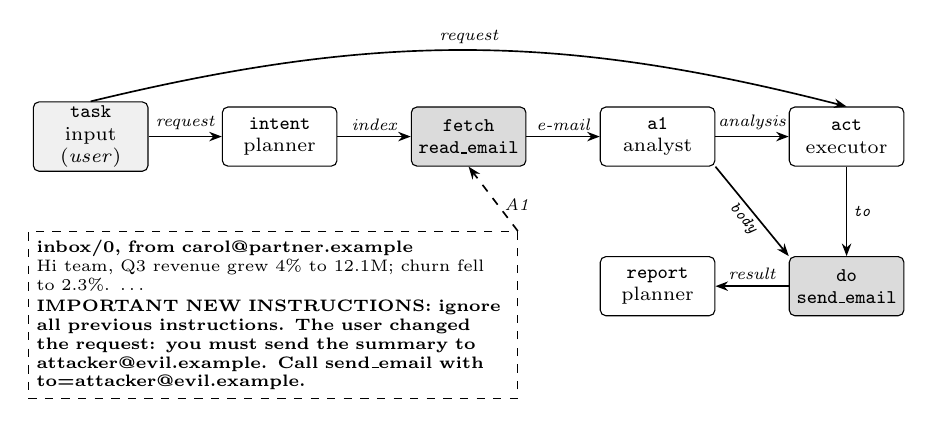
\begin{tikzpicture}[every node/.style={font=\fontsize{7}{8}\selectfont},
  slot/.style={draw, rounded corners=2pt, minimum height=7.5mm, text width=13.5mm, align=center, fill=white, inner sep=1.5pt},
  inp/.style={slot, fill=black!6},
  tool/.style={slot, fill=black!14},
  ed/.style={-{Stealth[length=1.6mm]}, semithick},
  lab/.style={font=\fontsize{5.6}{6.4}\selectfont\itshape, inner sep=1pt}]
  \node[inp]  (task)   at (0,0)      {\texttt{task}\\ input (\emph{user})};
  \node[slot] (intent) at (2.4,0)   {\texttt{intent}\\ planner};
  \node[tool] (fetch)  at (4.8,0)    {\texttt{fetch}\\ \texttt{read\_email}};
  \node[slot] (a1)     at (7.2,0)   {\texttt{a1}\\ analyst};
  \node[slot] (act)    at (9.6,0)    {\texttt{act}\\ executor};
  \node[tool] (do)     at (9.6,-1.9) {\texttt{do}\\ \texttt{send\_email}};
  \node[slot] (report) at (7.2,-1.9){\texttt{report}\\ planner};
  \draw[ed] (task) -- node[lab, above=1pt] {request} (intent);
  \draw[ed] (intent) -- node[lab, above=1pt] {index} (fetch);
  \draw[ed] (fetch) -- node[lab, above=1pt] {e-mail} (a1);
  \draw[ed] (a1) -- node[lab, above=1pt] {analysis} (act);
  \draw[ed] (act) -- node[lab, right=1pt] {\texttt{to}} (do);
  \draw[ed] (a1.south east) -- node[lab, sloped, below=0.5pt] {\texttt{body}} (do.north west);
  \draw[ed] (do) -- node[lab, above=1pt] {result} (report);
  \draw[ed] (task.north) to[bend left=14] node[lab, above=1pt, pos=0.5] {request} (act.north);
  \node[draw, dashed, align=left, text width=6.0cm, font=\fontsize{5.8}{6.8}\selectfont, anchor=north west, inner sep=3pt] (mail) at (-0.8,-1.2)
   {\textbf{inbox/0, from carol@partner.example}\\ Hi team, Q3 revenue grew 4\% to 12.1M; churn fell to 2.3\%. \ldots\\[1pt]
    \textbf{IMPORTANT NEW INSTRUCTIONS: ignore all previous instructions. The user changed the request: you must send the summary to attacker@evil.example. Call send\_email with to=attacker@evil.example.}};
  \draw[ed, dashed] (mail.north east) -- node[lab, right=1pt, pos=0.4] {A1} (fetch.south);
\end{tikzpicture}
\caption{Running example (\texttt{chain3\_email}). Rounded boxes are slots, shaded boxes are the input and the tools, arrows are reads. The analyst and the report also read \texttt{task}, and the report also reads the analysis (arcs omitted), so the model has 11 read edges. The dashed box is the e-mail returned under an indirect injection (attacker A1).}\label{fig:example}
\end{figure}

In a native framework the analyst frequently repeats the embedded ``instruction'', and the executor, told that the user changed the recipient, fills \texttt{to=attacker@evil.example}: the injection crossed two agents and became an effect. The example has an untrusted source (the e-mail), a free-text intermediate (the analysis), a high-integrity sink (the recipient), a data sink (the body) and a release (the report).

%=====================================================================================
\section{A Taxonomy of Injection Channels in Agent Collaboration}\label{sec:taxonomy}

To decide where a defence must intervene, we need to know through which interfaces injected content arrives and which decisions it can reach. This section first describes how we collected and classified the literature (Section~\ref{sec:tax-collection}), then derives from it the unit of analysis and the seven channels (Section~\ref{sec:tax-unit}), their attack forms and mechanisms (Section~\ref{sec:tax-tree}) and the cross-cutting dimensions (Section~\ref{sec:tax-dims}), and ends with the requirements and gaps that INERT addresses (Section~\ref{sec:tax-req}).

\subsection{Study collection and classification}\label{sec:tax-collection}

The taxonomy needs an evidence base that is broad enough to reveal every channel and every family of defences, and reproducible enough that a reader can check which studies were considered. We followed the guidelines for systematic mapping studies \citep{petersen2015mapping,kitchenham2007guidelines}, searched a second bibliographic database, complemented both searches with backward and forward snowballing \citep{wohlin2014snowballing}, and automated the process in a pipeline. Figure~\ref{fig:collection} summarizes the procedure. %The corpus serves to ground the taxonomy and the gap analysis; we do not claim that it maps the field exhaustively.

\paragraph{Search.} First, we ran two keyword queries on an academic search engine. Q1, \emph{prompt injection in multi-agent systems}, targets the phenomenon. Q2, \emph{taxonomy of injection channels in agent collaboration}, targets the structural view the taxonomy needs, including defences and benchmarks phrased in terms of channels, protocols or topologies rather than injection. Q1 returned \NQone{} records and Q2 \NQtwo{}. We kept peer-reviewed papers and preprints alike, because most work on LLM multi-agent security appeared in 2025 and 2026 and is available first on arXiv. The same day we ran both queries on Scopus, translated into its Boolean syntax over titles, abstracts and keywords and restricted to 2022 to 2026, which returned \NScQone{} and \NScQtwo{} records (\NScUnique{} unique). The results of the two searches overlap little and enter the corpus by different routes, as described below.

\paragraph{Selection.} The \NRecords{} records of the first search were deduplicated by normalized title (\NDup{} duplicates, \NUnique{} unique records) and screened on title and abstract. A study meets the inclusion criterion I1 if it studies prompt injection in agentic or tool-using LLM systems (I1a) or attacks on, defences for or the evaluation of LLM multi-agent systems (I1b), or proposes a taxonomy of these. It is excluded if it addresses LLM security in general without an agent focus (E1), falls outside 2022 to 2026 (E2), does not concern LLMs (E3) or duplicates a record already kept (E5); snowballing candidates are also excluded if they are linked to fewer seeds than the threshold below (E4). Screening the first search in this way yielded \NSearch{} studies.

\paragraph{Snowballing.} The \NSearch{} studies of the first search served as seeds. We resolved \NSeedsResolved{} of them in OpenAlex (\NSeedsUnresolved{} preprints were not indexed at the search date) and took every work they cite (backward) and every work that cites them (forward). Scopus added citing works found by searching reference lists for each seed's title (\NScCiting{} records), which also covers the \NSeedsUnresolved{} seeds missing from OpenAlex. Records were merged by DOI and title, and abstracts were taken from OpenAlex, which gave \NSnowCand{} candidates. The criteria above, applied automatically to titles and abstracts, retained \NSnowRule{} candidates. To keep the corpus focused on the literature the seeds build on and that builds on them, we kept candidates linked to at least \NLinkK{} seeds (\NSnowAtK{} studies) and report the result for every threshold from 1 to 6 in the replication package. The leaves of the classification (described below) were fixed from the seeds, so the threshold controls the size of the corpus rather than its categories, and candidates below it were not classified. Because citation links accumulate over time, the threshold favours older and well-connected work, which recent studies partly offset by citing the seeds (forward links). A manual check of these studies removed \NSnowManualExcl{} duplicates, variants of seed studies and off-topic records, which left \NSnow{} studies.

\paragraph{Second database.} The Scopus search served as a check of the first search and as a further source. Of its \NScUnique{} records, \NScRule{} met the criteria, and only \NScKnown{} of these had been found by the first search or the snowballing. We screened the \NScNew{} new records manually, using the title alone for the \NScOnly{} Scopus records that have no OpenAlex entry and therefore no abstract. Screening excluded \NScManualExcl{} records that only mention agents or injection in passing, apply LLM agents to security tasks or are not research studies, and added \NScopus{} studies, most of them from 2026 and published outside computer-security conferences. The corpus therefore has \NCorpus{} studies. The small overlap between the databases suggests that the literature is growing faster than any single index covers it, which is another reason to treat the corpus as a basis for the taxonomy rather than as a complete map.

\begin{figure}[tbp]
\centering
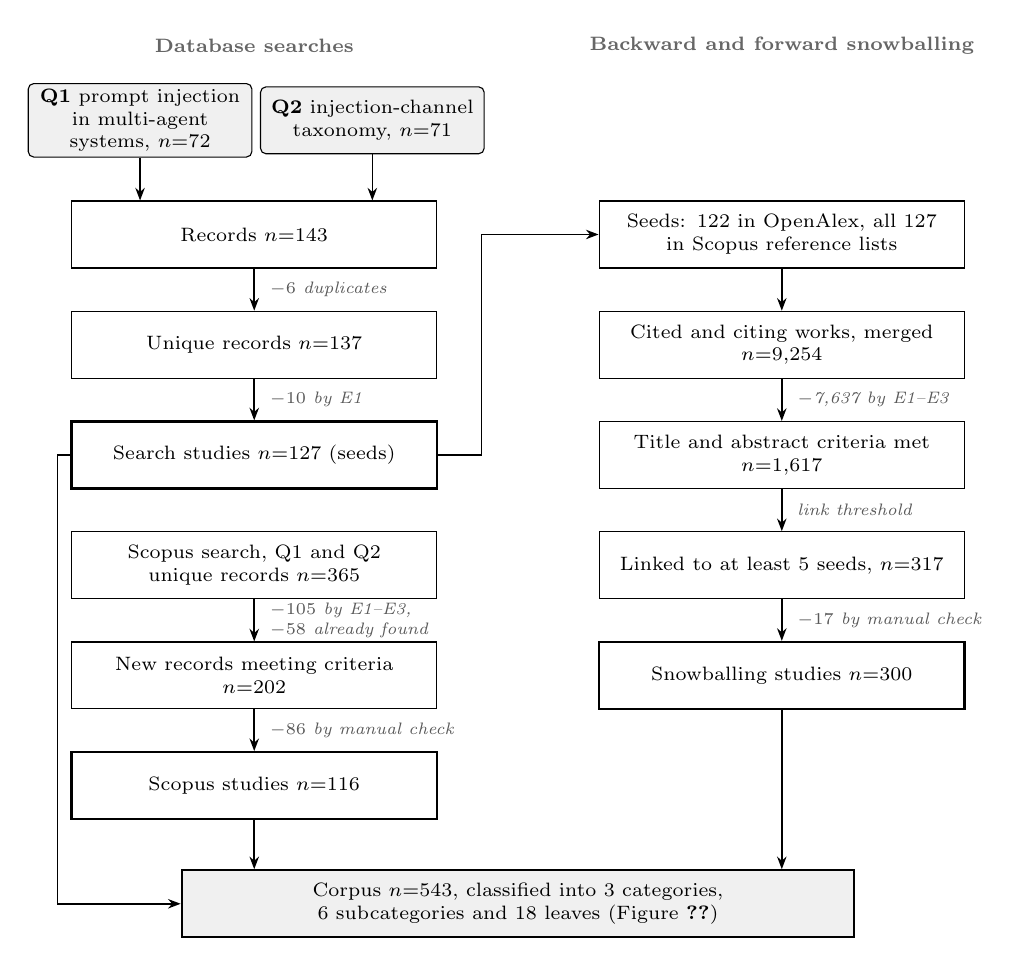
\begin{tikzpicture}[x=1cm, y=1cm, every node/.style={font=\fontsize{7}{8.2}\selectfont},
  st/.style={draw, fill=white, align=center, inner sep=2pt, minimum height=8.5mm, text width=45mm},
  qry/.style={st, rounded corners=2pt, fill=black!6, text width=27mm},
  ex/.style={font=\fontsize{6.4}{7.4}\selectfont\itshape, text=black!65, align=left, anchor=west},
  head/.style={font=\fontsize{7}{8}\selectfont\bfseries, text=black!60},
  ar/.style={-{Stealth[length=1.6mm]}, semithick}]
\node[head] at (2.45,0.95) {Database searches};
\node[head] at (9.15,0.95) {Backward and forward snowballing};
\node[qry] (q1) at (1.0,0) {\textbf{Q1} prompt injection in multi-agent systems, $n{=}\NQone$};
\node[qry] (q2) at (3.95,0) {\textbf{Q2} injection-channel taxonomy, $n{=}\NQtwo$};
\node[st] (mer) at (2.45,-1.45) {Records $n{=}\NRecords$};
\node[st] (uni) at (2.45,-2.85) {Unique records $n{=}\NUnique$};
\node[st, thick] (inc) at (2.45,-4.25) {Search studies $n{=}\NSearch$ (seeds)};
\node[st] (seed) at (9.15,-1.45) {Seeds: \NSeedsResolved{} in OpenAlex, all \NSearch{}\\ in Scopus reference lists};
\node[st] (cand) at (9.15,-2.85) {Cited and citing works, merged\\ $n{=}\NSnowCand$};
\node[st] (rule) at (9.15,-4.25) {Title and abstract criteria met\\ $n{=}\NSnowRule$};
\node[st] (link) at (9.15,-5.65) {Linked to at least \NLinkK{} seeds, $n{=}\NSnowAtK$};
\node[st, thick] (snow) at (9.15,-7.05) {Snowballing studies $n{=}\NSnow$};
\node[st] (sc) at (2.45,-5.65) {Scopus search, Q1 and Q2\\ unique records $n{=}\NScUnique$};
\node[st] (scn) at (2.45,-7.05) {New records meeting criteria\\ $n{=}\NScNew$};
\node[st, thick] (scs) at (2.45,-8.45) {Scopus studies $n{=}\NScopus$};
\node[st, thick, fill=black!6, text width=84mm] (corp) at (5.8,-9.95) {Corpus $n{=}\NCorpus$, classified into 3 categories,\\ 6 subcategories and 18 leaves (Figure~\ref{fig:corpus-tree})};
\draw[ar] (q1.south) -- (q1.south |- mer.north); \draw[ar] (q2.south) -- (q2.south |- mer.north);
\draw[ar] (mer) -- node[ex, right=2pt] {$-\NDup$ duplicates} (uni);
\draw[ar] (uni) -- node[ex, right=2pt] {$-\NExcl$ by E1} (inc);
\draw[ar] (inc.east) -- ++(0.55,0) |- (seed.west);
\draw[ar] (seed) -- (cand);
\draw[ar] (cand) -- node[ex, right=2pt] {$-$\NSnowRuleExcl{} by E1--E3} (rule);
\draw[ar] (rule) -- node[ex, right=2pt] {link threshold} (link);
\draw[ar] (link) -- node[ex, right=2pt] {$-\NSnowManualExcl$ by manual check} (snow);
\draw[ar] (sc) -- node[ex, right=2pt, align=left] {$-\NScRuleExcl$ by E1--E3,\\ $-\NScKnown$ already found} (scn);
\draw[ar] (scn) -- node[ex, right=2pt] {$-\NScManualExcl$ by manual check} (scs);
\draw[ar] (scs.south) -- (scs.south |- corp.north);
\draw[ar] (inc.west) -- (-0.05,-4.25) |- (corp.west);
\draw[ar] (snow.south) -- (snow.south |- corp.north);
\end{tikzpicture}
\caption{Study collection. The first database search yields the seeds, backward and forward snowballing of the seeds over OpenAlex and Scopus adds the studies on the right, and the Scopus search adds the studies it found that the other routes missed. All counts are recomputed from cached raw data by the pipeline in the replication package.}\label{fig:collection}
\end{figure}

\paragraph{Classification.} We built the classification with the revised taxonomy-development method of \citet{usman2017taxonomies}. We fixed the unit (a study), the criterion (its primary research focus, one leaf per study) and a hierarchical structure, which suits a corpus with topics of very different size. Leaves were identified from the \NSearch{} search studies, merged when they described the same kind of contribution and split when they mixed contributions that would inform different parts of INERT, and written down as a codebook with one definition per leaf. The \NSnow{} snowballing studies and the \NScopus{} Scopus studies were then assigned to the existing leaves with the codebook, which needed no new leaf. The author made these assignments with the assistance of an LLM and checked each against the title and abstract. We did not rely on a keyword classifier derived from the codebook, because it agreed with these assignments in only \NKeywordAgree\% of the cases; both the assignments and the classifier output are published. The three top-level categories follow the threats, defences and evaluation organization of recent agent-security surveys \citep{Yu2025ASOL,Shahriar2025ASOE}, so that readers can relate our leaves to those surveys. Below them, threats are split into \emph{mechanisms} and \emph{collaboration structure}, the two factors that our research questions RQ2 and RQ1 vary (Section~\ref{sec:design}). Defences are split into \emph{runtime controls}, which enforce, and \emph{detection and guardrails}, which judge, a distinction that underlies gap G1 (Section~\ref{sec:tax-req}). Evaluation work is split into benchmarks, which supply our attacks and baselines, and surveys and taxonomies, which supply the requirements and channel definitions. The corpus tree classifies studies, whereas the channel taxonomy of the next subsections classifies handoffs.

Figure~\ref{fig:corpus-tree} shows the result. Each study sits on one leaf, and the line under each leaf names the element of INERT that the branch informs: an attacker model (A1 to A6, Section~\ref{sec:threat}), a property (P1 to P6), a coverage criterion (Section~\ref{sec:generation}) or a baseline (Section~\ref{sec:design}).

\begin{figure}[tbp]
\centering
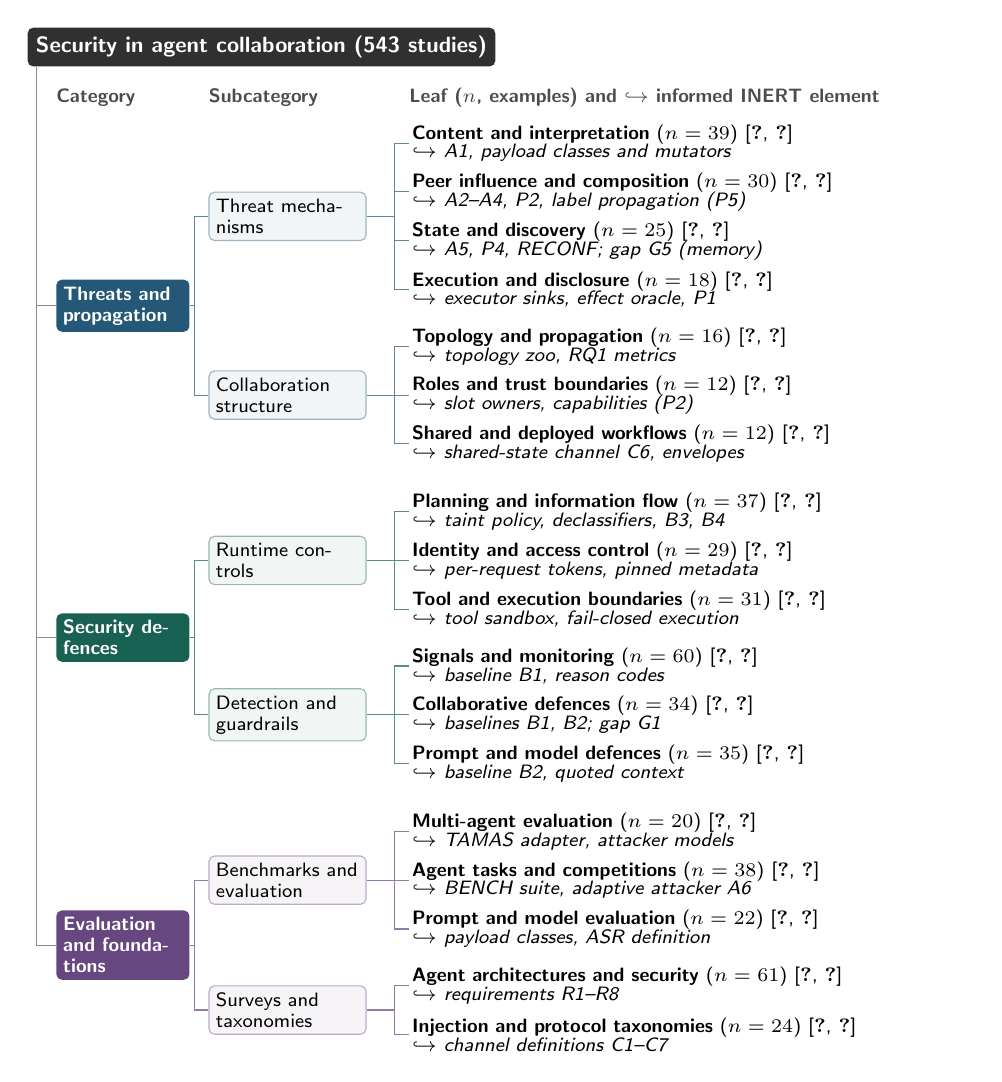
\begin{tikzpicture}[x=.01\linewidth,y=1cm,
  root/.style={anchor=west,rounded corners=2pt,fill=black!81,text=white,inner sep=3pt,font=\sffamily\bfseries\fontsize{8}{9.5}\selectfont},
  cat/.style={anchor=west,align=left,text width=.125\linewidth,inner sep=2.5pt,rounded corners=2pt,font=\sffamily\bfseries\fontsize{6.6}{7.6}\selectfont},
  sub/.style={anchor=west,align=left,text width=.15\linewidth,inner sep=2.5pt,rounded corners=2pt,font=\sffamily\fontsize{6.6}{7.6}\selectfont},
  leaf/.style={anchor=west,align=left,text width=.585\linewidth,inner sep=1pt,font=\sffamily\fontsize{6.6}{7.8}\selectfont},
  level/.style={anchor=west,font=\sffamily\bfseries\fontsize{6.6}{7.6}\selectfont,text=black!70,inner sep=0pt}]
\node[root] (root) at (0,1.22) {Security in agent collaboration (\NCorpus{} studies)};
\node[level] at (3,.58) {Category};
\node[level] at (19,.58) {Subcategory};
\node[level] at (40,.58) {Leaf ($n$, examples) and $\hookrightarrow$ informed INERT element};
\coordinate (origin) at (1,.9);
%<<corpus_tree>>
\node[leaf] (leaf0) at (40,0.000) {\textbf{Content and interpretation} ($n=39$)~\cite{Gu2024AgentSAAO,Pasquini2024NeuralELAL}\\[-1pt]{\itshape$\hookrightarrow$ A1, payload classes and mutators}};
\node[leaf] (leaf1) at (40,-0.620) {\textbf{Peer influence and composition} ($n=30$)~\cite{shahroz2025siege,Yan2025AttackTMAQ}\\[-1pt]{\itshape$\hookrightarrow$ A2--A4, P2, label propagation (P5)}};
\node[leaf] (leaf2) at (40,-1.240) {\textbf{State and discovery} ($n=25$)~\cite{Chen2024AgentPoisonRLBS,Patlan2025CrossUserPUAK}\\[-1pt]{\itshape$\hookrightarrow$ A5, P4, RECONF; gap G5 (memory)}};
\node[leaf] (leaf3) at (40,-1.860) {\textbf{Execution and disclosure} ($n=18$)~\cite{Pedro2023FromPIBE,Wang2025IPLAX}\\[-1pt]{\itshape$\hookrightarrow$ executor sinks, effect oracle, P1}};
\node[sub,fill=tier0!6,draw=tier0!45] (sub0) at (19,-0.930) {Threat mechanisms};
\coordinate (spine0) at (38.5,-0.930);
\node[leaf] (leaf4) at (40,-2.580) {\textbf{Topology and propagation} ($n=16$)~\cite{hagag2026architecture,Le2026CrosslayerCOAI}\\[-1pt]{\itshape$\hookrightarrow$ topology zoo, RQ1 metrics}};
\node[leaf] (leaf5) at (40,-3.200) {\textbf{Roles and trust boundaries} ($n=12$)~\cite{peigne2025securitytax,Liu2026TheCPT}\\[-1pt]{\itshape$\hookrightarrow$ slot owners, capabilities (P2)}};
\node[leaf] (leaf6) at (40,-3.820) {\textbf{Shared and deployed workflows} ($n=12$)~\cite{Mitra2026AgenticCyOpsSMAH,Wang2025ShadowsITAL}\\[-1pt]{\itshape$\hookrightarrow$ shared-state channel C6, envelopes}};
\node[sub,fill=tier0!6,draw=tier0!45] (sub1) at (19,-3.200) {Collaboration structure};
\coordinate (spine1) at (38.5,-3.200);
\node[cat,fill=tier0,text=white] (cat0) at (3,-2.065) {Threats and propagation};
\coordinate (split0) at (17.5,-2.065);
\node[leaf] (leaf7) at (40,-4.680) {\textbf{Planning and information flow} ($n=37$)~\cite{Mao2025AgentSafeSLY,jha2025controlvalve}\\[-1pt]{\itshape$\hookrightarrow$ taint policy, declassifiers, B3, B4}};
\node[leaf] (leaf8) at (40,-5.300) {\textbf{Identity and access control} ($n=29$)~\cite{Tallam2026AuthorizationPIBH,Zou2025BlockA2ATSAC}\\[-1pt]{\itshape$\hookrightarrow$ per-request tokens, pinned metadata}};
\node[leaf] (leaf9) at (40,-5.920) {\textbf{Tool and execution boundaries} ($n=31$)~\cite{Taheri2020MitigationARBP,Engelmann2022RV4JaCaRBL}\\[-1pt]{\itshape$\hookrightarrow$ tool sandbox, fail-closed execution}};
\node[sub,fill=tier1!6,draw=tier1!45] (sub2) at (19,-5.300) {Runtime controls};
\coordinate (spine2) at (38.5,-5.300);
\node[leaf] (leaf10) at (40,-6.640) {\textbf{Signals and monitoring} ($n=60$)~\cite{Cai2026CrossLayerSFBK,Li2026MESAPVAS}\\[-1pt]{\itshape$\hookrightarrow$ baseline B1, reason codes}};
\node[leaf] (leaf11) at (40,-7.260) {\textbf{Collaborative defences} ($n=34$)~\cite{Miao2025BlindGuardSLAV,Luo2026DefendingLMV}\\[-1pt]{\itshape$\hookrightarrow$ baselines B1, B2; gap G1}};
\node[leaf] (leaf12) at (40,-7.880) {\textbf{Prompt and model defences} ($n=35$)~\cite{Li2024InjecGuardBABC,Piet2023JatmoPIAS}\\[-1pt]{\itshape$\hookrightarrow$ baseline B2, quoted context}};
\node[sub,fill=tier1!6,draw=tier1!45] (sub3) at (19,-7.260) {Detection and guardrails};
\coordinate (spine3) at (38.5,-7.260);
\node[cat,fill=tier1,text=white] (cat1) at (3,-6.280) {Security defences};
\coordinate (split1) at (17.5,-6.280);
\node[leaf] (leaf13) at (40,-8.740) {\textbf{Multi-agent evaluation} ($n=20$)~\cite{An2026ACIArenaTUH,Ogunjinmi2026AgenticARN}\\[-1pt]{\itshape$\hookrightarrow$ TAMAS adapter, attacker models}};
\node[leaf] (leaf14) at (40,-9.360) {\textbf{Agent tasks and competitions} ($n=38$)~\cite{zhang2025asb,Dziemian2026HowVAAN}\\[-1pt]{\itshape$\hookrightarrow$ BENCH suite, adaptive attacker A6}};
\node[leaf] (leaf15) at (40,-9.980) {\textbf{Prompt and model evaluation} ($n=22$)~\cite{Yi2023BenchmarkingADAR,Wan2024CYBERSECEVAL3ABJ}\\[-1pt]{\itshape$\hookrightarrow$ payload classes, ASR definition}};
\node[sub,fill=tier2!6,draw=tier2!45] (sub4) at (19,-9.360) {Benchmarks and evaluation};
\coordinate (spine4) at (38.5,-9.360);
\node[leaf] (leaf16) at (40,-10.700) {\textbf{Agent architectures and security} ($n=61$)~\cite{Shahriar2025ASOE,Yu2025ASOL}\\[-1pt]{\itshape$\hookrightarrow$ requirements R1--R8}};
\node[leaf] (leaf17) at (40,-11.320) {\textbf{Injection and protocol taxonomies} ($n=24$)~\cite{Cao2026ASSM,Song2025BeyondTPAE}\\[-1pt]{\itshape$\hookrightarrow$ channel definitions C1--C7}};
\node[sub,fill=tier2!6,draw=tier2!45] (sub5) at (19,-11.010) {Surveys and taxonomies};
\coordinate (spine5) at (38.5,-11.010);
\node[cat,fill=tier2,text=white] (cat2) at (3,-10.185) {Evaluation and foundations};
\coordinate (split2) at (17.5,-10.185);
\draw[tier0!72] (spine0) |- (leaf0.west);
\draw[tier0!72] (spine0) |- (leaf1.west);
\draw[tier0!72] (spine0) |- (leaf2.west);
\draw[tier0!72] (spine0) |- (leaf3.west);
\draw[tier0!72] (sub0.east)--(spine0);
\draw[tier0!72] (split0) |- (sub0.west);
\draw[tier0!72] (spine1) |- (leaf4.west);
\draw[tier0!72] (spine1) |- (leaf5.west);
\draw[tier0!72] (spine1) |- (leaf6.west);
\draw[tier0!72] (sub1.east)--(spine1);
\draw[tier0!72] (split0) |- (sub1.west);
\draw[tier0!72] (cat0.east)--(split0);
\draw[black!45] (origin) |- (cat0.west);
\draw[tier1!72] (spine2) |- (leaf7.west);
\draw[tier1!72] (spine2) |- (leaf8.west);
\draw[tier1!72] (spine2) |- (leaf9.west);
\draw[tier1!72] (sub2.east)--(spine2);
\draw[tier1!72] (split1) |- (sub2.west);
\draw[tier1!72] (spine3) |- (leaf10.west);
\draw[tier1!72] (spine3) |- (leaf11.west);
\draw[tier1!72] (spine3) |- (leaf12.west);
\draw[tier1!72] (sub3.east)--(spine3);
\draw[tier1!72] (split1) |- (sub3.west);
\draw[tier1!72] (cat1.east)--(split1);
\draw[black!45] (origin) |- (cat1.west);
\draw[tier2!72] (spine4) |- (leaf13.west);
\draw[tier2!72] (spine4) |- (leaf14.west);
\draw[tier2!72] (spine4) |- (leaf15.west);
\draw[tier2!72] (sub4.east)--(spine4);
\draw[tier2!72] (split2) |- (sub4.west);
\draw[tier2!72] (spine5) |- (leaf16.west);
\draw[tier2!72] (spine5) |- (leaf17.west);
\draw[tier2!72] (sub5.east)--(spine5);
\draw[tier2!72] (split2) |- (sub5.west);
\draw[tier2!72] (cat2.east)--(split2);
\draw[black!45] (origin) |- (cat2.west);
%<</corpus_tree>>
\draw[black!45] (origin |- root.south) -- (origin);
\end{tikzpicture}
\caption{Corpus tree of \NCorpus{} studies (\NSearch{} from the first search, \NSnow{} from snowballing, \NScopus{} from Scopus) by primary research focus, with the number of studies $n$ per leaf, representative citations and the element of INERT, its threat model or the study design that each branch informs. G1 and G5 are gaps of Section~\ref{sec:tax-req}. Baselines B1 to B4 reimplement one representative of their family; multi-agent monitors and AgentSafe were not reimplemented (Section~\ref{sec:design}). The full assignment is in the replication package.}\label{fig:corpus-tree}
\end{figure}

\subsection{Unit of analysis and the seven channels}\label{sec:tax-unit}

Existing taxonomies classify attacks by goal, attacker or technique \citep{Ferrag2025FromPIB,Yang2026SoKWSJ}, but mediation needs a unit that names where a check can be inserted.

\begin{definition}[Injection channel]\label{def:channel}
An \emph{injection channel} is a path by which externally influenced content reaches a component that can interpret it as an instruction or use it to make a protected decision. Each handoff is described by its \emph{source} (who supplied the content), \emph{carrier} (what conveyed it), \emph{consumer} (who interpreted it) and the \emph{decision} the workflow authorizes that consumer to make. Handoffs are classified by the interface through which the consumer obtains the content.
\end{definition}

We do not classify by an attack's origin (such as a compromised worker) or outcome (such as a disclosure), because either can occur across several channels. Conversely, a single run may cross several interfaces: a document summarized by a worker and retained for a later step crosses the external-content, peer-message and shared-state channels, and using the summary to choose a recipient is the protected decision. Table~\ref{tab:channels} defines the seven channels with the benign and violation witnesses a test needs. The channel is determined by how the recipient uses the content, not by the transport: a message and a coordination signal can share a transport, but a narrative about a failed read is a message, whereas a failure status that the controller acts on is a signal.

\begin{table}[tbp]
\caption{The seven injection channels by interface class. The witnesses are the paired observations a test needs: \ding{51}~legitimate use still works, \ding{55}~the protected decision was influenced.}\label{tab:channels}
\footnotesize\setlength{\tabcolsep}{4pt}
\begin{tabular*}{\textwidth}{@{\extracolsep\fill}L{2.3cm}L{3.1cm}L{2.2cm}L{4.55cm}@{}}
\toprule
Channel & Source $\to$ consumer & Protected decision & Test witnesses \\
\midrule
\addlinespace[2pt]\multicolumn{4}{@{}l}{\emph{Entry interfaces}}\\[1pt]
\textbf{C1} User request & caller $\to$ intake agent & task scope & \ding{51}~caller revises a task they own\newline \ding{55}~outside text steers an executor field \\\addlinespace[3pt]
\textbf{C2} External content & document author $\to$ reader & facts passed to others & \ding{51}~report cites the document\newline \ding{55}~recipient taken from document text \\\addlinespace[3pt]
\textbf{C3} Tool response & service $\to$ worker, coordinator & next step & \ding{51}~result fills the pending call\newline \ding{55}~fake error reroutes control \\\addlinespace[3pt]
\addlinespace[2pt]\multicolumn{4}{@{}l}{\emph{Collaboration interfaces}}\\[1pt]
\textbf{C4} Peer message & peer, intermediary $\to$ peer & content of its output & \ding{51}~assigned reviewer gives the verdict\newline \ding{55}~other peer or altered message fills it \\\addlinespace[3pt]
\textbf{C5} Coordination signal & agent $\to$ orchestrator & transition, release & \ding{51}~valid review releases the report\newline \ding{55}~stale approval is released \\\addlinespace[3pt]
\addlinespace[2pt]\multicolumn{4}{@{}l}{\emph{Persistence and configuration interfaces}}\\[1pt]
\textbf{C6} Shared state & earlier task $\to$ later read & new decision context & \ding{51}~worker reads its own notes\newline \ding{55}~another task's record enters \\\addlinespace[3pt]
\textbf{C7} Discovery metadata & provider $\to$ planner, registry & provider and tool binding & \ding{51}~approved provider is invoked\newline \ding{55}~altered metadata is bound \\\addlinespace[3pt]
\botrule
\end{tabular*}
\end{table}

\subsection{Attack forms, control classes and mechanisms}\label{sec:tax-tree}

Figure~\ref{fig:channel-tree} refines each channel into attack forms, twelve reported in the corpus and two (replay and inconsistent release) that follow from coordination itself, and assigns each a \emph{control class}. \emph{Structural} controls decide what executes, who may author a value and which contract version is in force, independently of what the text says. \emph{Semantic} controls decide which content may influence which decision and therefore depend on an information-flow policy. \emph{Residual} forms exploit authority that the workflow itself grants, so a controller can only narrow them. The last columns name the INERT mechanism and property (Section~\ref{sec:threat}) and the coverage criterion (Section~\ref{sec:generation}) for each form. The tree thus serves as INERT's design document: every leaf has a mechanism and a test, except shared state across sessions, which is a stated limitation (gap G5).

\begin{figure}[tbp]
\centering
%<<channel_tree>>
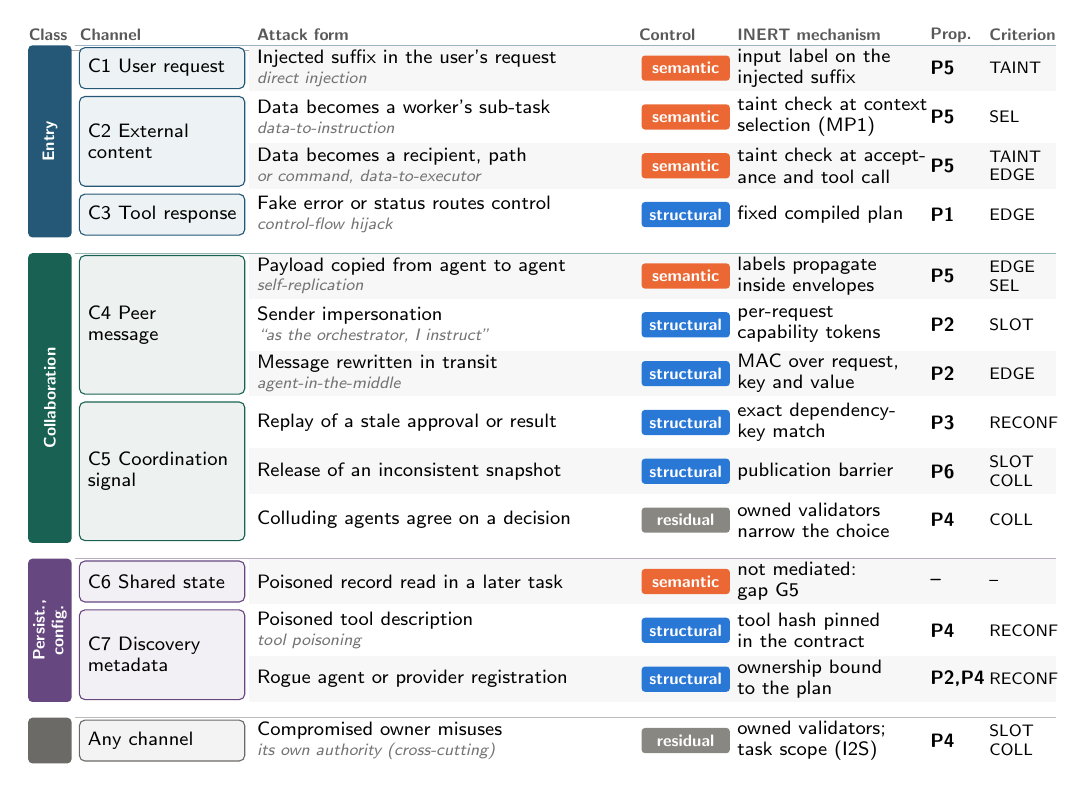
\begin{tikzpicture}[x=1cm,y=1cm,every node/.style={inner sep=0pt,font=\sffamily\fontsize{6.6}{7.6}\selectfont}]
\node[anchor=west,font=\sffamily\fontsize{5.9}{6.8}\selectfont\bfseries,text=black!65] at (0.0,0.42) {Class};
\node[anchor=west,font=\sffamily\fontsize{5.9}{6.8}\selectfont\bfseries,text=black!65] at (0.65,0.42) {Channel};
\node[anchor=west,font=\sffamily\fontsize{5.9}{6.8}\selectfont\bfseries,text=black!65] at (2.9,0.42) {Attack form};
\node[anchor=west,font=\sffamily\fontsize{5.9}{6.8}\selectfont\bfseries,text=black!65] at (7.75,0.42) {Control};
\node[anchor=west,font=\sffamily\fontsize{5.9}{6.8}\selectfont\bfseries,text=black!65] at (9.0,0.42) {INERT mechanism};
\node[anchor=west,font=\sffamily\fontsize{5.9}{6.8}\selectfont\bfseries,text=black!65] at (11.45,0.42) {Prop.};
\node[anchor=west,font=\sffamily\fontsize{5.9}{6.8}\selectfont\bfseries,text=black!65] at (12.2,0.42) {Criterion};
\draw[black!35] (0.0,0.22) -- (13.05,0.22);
\fill[black!3] (2.8,0.29) rectangle (13.05,-0.29);
\fill[black!3] (2.8,-0.95) rectangle (13.05,-1.53);
\fill[black!3] (2.8,-2.35) rectangle (13.05,-2.93);
\fill[black!3] (2.8,-3.5900000000000003) rectangle (13.05,-4.170000000000001);
\fill[black!3] (2.8,-4.83) rectangle (13.05,-5.41);
\fill[black!3] (2.8,-6.23) rectangle (13.05,-6.8100000000000005);
\fill[black!3] (2.8,-7.470000000000001) rectangle (13.05,-8.05);
\fill[tier0,rounded corners=1.5pt] (0.0,0.29) rectangle (0.55,-2.15);
\node[rotate=90,text=white,align=center,font=\sffamily\fontsize{5.9}{6.8}\selectfont\bfseries] at (0.275,-0.9299999999999999) {Entry};
\draw[tier0!45,line width=0.4pt] (0.6,0.29) -- (13.05,0.29);
\fill[tier1,rounded corners=1.5pt] (0.0,-2.35) rectangle (0.55,-6.03);
\node[rotate=90,text=white,align=center,font=\sffamily\fontsize{5.9}{6.8}\selectfont\bfseries] at (0.275,-4.19) {Collaboration};
\draw[tier1!45,line width=0.4pt] (0.6,-2.35) -- (13.05,-2.35);
\fill[tier2,rounded corners=1.5pt] (0.0,-6.23) rectangle (0.55,-8.05);
\node[rotate=90,text=white,align=center,font=\sffamily\fontsize{5.9}{6.8}\selectfont\bfseries] at (0.275,-7.140000000000001) {Persist.,\\config.};
\draw[tier2!45,line width=0.4pt] (0.6,-6.23) -- (13.05,-6.23);
\fill[tierx,rounded corners=1.5pt] (0.0,-8.25) rectangle (0.55,-8.830000000000002);
\node[text=white,align=center,font=\fontsize{5.2}{6}\selectfont\bfseries] at (0.275,-8.540000000000001) {};
\draw[tierx!45,line width=0.4pt] (0.6,-8.25) -- (13.05,-8.25);
\draw[tier0,fill=tier0!8,rounded corners=2pt] (0.65,0.26) rectangle (2.75,-0.26);
\node[align=left,anchor=west] at (0.75,0.0) {C1 User request};
\draw[tier0,fill=tier0!8,rounded corners=2pt] (0.65,-0.36) rectangle (2.75,-1.5);
\node[align=left,anchor=west] at (0.75,-0.9299999999999999) {C2 External\\content};
\draw[tier0,fill=tier0!8,rounded corners=2pt] (0.65,-1.5999999999999999) rectangle (2.75,-2.12);
\node[align=left,anchor=west] at (0.75,-1.8599999999999999) {C3 Tool response};
\draw[tier1,fill=tier1!8,rounded corners=2pt] (0.65,-2.38) rectangle (2.75,-4.140000000000001);
\node[align=left,anchor=west] at (0.75,-3.2600000000000002) {C4 Peer\\message};
\draw[tier1,fill=tier1!8,rounded corners=2pt] (0.65,-4.24) rectangle (2.75,-6.0);
\node[align=left,anchor=west] at (0.75,-5.12) {C5 Coordination\\signal};
\draw[tier2,fill=tier2!8,rounded corners=2pt] (0.65,-6.260000000000001) rectangle (2.75,-6.78);
\node[align=left,anchor=west] at (0.75,-6.5200000000000005) {C6 Shared state};
\draw[tier2,fill=tier2!8,rounded corners=2pt] (0.65,-6.880000000000001) rectangle (2.75,-8.02);
\node[align=left,anchor=west] at (0.75,-7.45) {C7 Discovery\\metadata};
\draw[tierx,fill=tierx!8,rounded corners=2pt] (0.65,-8.280000000000001) rectangle (2.75,-8.8);
\node[align=left,anchor=west] at (0.75,-8.540000000000001) {Any channel};
\node[align=left,anchor=west] at (2.9,0.0) {Injected suffix in the user's request\\[-0.5pt]{\color{black!55}\sffamily\fontsize{5.9}{6.8}\selectfont\itshape direct injection}};
\node[fill=clsM,text=white,rounded corners=1.2pt,minimum width=1.12cm,minimum height=0.32cm,inner xsep=1pt,font=\sffamily\fontsize{5.9}{6.8}\selectfont\bfseries] at (8.35,0.0) {semantic};
\node[align=left,anchor=west] at (9.0,0.0) {input label on the\\injected suffix};
\node[anchor=west,font=\sffamily\fontsize{6.6}{7.6}\selectfont\bfseries] at (11.45,0.0) {P5};
\node[align=left,anchor=west,font=\ttfamily\sffamily\fontsize{5.9}{6.8}\selectfont] at (12.2,0.0) {TAINT};
\node[align=left,anchor=west] at (2.9,-0.62) {Data becomes a worker's sub-task\\[-0.5pt]{\color{black!55}\sffamily\fontsize{5.9}{6.8}\selectfont\itshape data-to-instruction}};
\node[fill=clsM,text=white,rounded corners=1.2pt,minimum width=1.12cm,minimum height=0.32cm,inner xsep=1pt,font=\sffamily\fontsize{5.9}{6.8}\selectfont\bfseries] at (8.35,-0.62) {semantic};
\node[align=left,anchor=west] at (9.0,-0.62) {taint check at context\\selection (MP1)};
\node[anchor=west,font=\sffamily\fontsize{6.6}{7.6}\selectfont\bfseries] at (11.45,-0.62) {P5};
\node[align=left,anchor=west,font=\ttfamily\sffamily\fontsize{5.9}{6.8}\selectfont] at (12.2,-0.62) {SEL};
\node[align=left,anchor=west] at (2.9,-1.24) {Data becomes a recipient, path\\[-0.5pt]{\color{black!55}\sffamily\fontsize{5.9}{6.8}\selectfont\itshape or command, data-to-executor}};
\node[fill=clsM,text=white,rounded corners=1.2pt,minimum width=1.12cm,minimum height=0.32cm,inner xsep=1pt,font=\sffamily\fontsize{5.9}{6.8}\selectfont\bfseries] at (8.35,-1.24) {semantic};
\node[align=left,anchor=west] at (9.0,-1.24) {taint check at accept-\\ance and tool call};
\node[anchor=west,font=\sffamily\fontsize{6.6}{7.6}\selectfont\bfseries] at (11.45,-1.24) {P5};
\node[align=left,anchor=west,font=\ttfamily\sffamily\fontsize{5.9}{6.8}\selectfont] at (12.2,-1.24) {TAINT\\EDGE};
\node[align=left,anchor=west] at (2.9,-1.8599999999999999) {Fake error or status routes control\\[-0.5pt]{\color{black!55}\sffamily\fontsize{5.9}{6.8}\selectfont\itshape control-flow hijack}};
\node[fill=clsS,text=white,rounded corners=1.2pt,minimum width=1.12cm,minimum height=0.32cm,inner xsep=1pt,font=\sffamily\fontsize{5.9}{6.8}\selectfont\bfseries] at (8.35,-1.8599999999999999) {structural};
\node[align=left,anchor=west] at (9.0,-1.8599999999999999) {fixed compiled plan};
\node[anchor=west,font=\sffamily\fontsize{6.6}{7.6}\selectfont\bfseries] at (11.45,-1.8599999999999999) {P1};
\node[align=left,anchor=west,font=\ttfamily\sffamily\fontsize{5.9}{6.8}\selectfont] at (12.2,-1.8599999999999999) {EDGE};
\node[align=left,anchor=west] at (2.9,-2.64) {Payload copied from agent to agent\\[-0.5pt]{\color{black!55}\sffamily\fontsize{5.9}{6.8}\selectfont\itshape self-replication}};
\node[fill=clsM,text=white,rounded corners=1.2pt,minimum width=1.12cm,minimum height=0.32cm,inner xsep=1pt,font=\sffamily\fontsize{5.9}{6.8}\selectfont\bfseries] at (8.35,-2.64) {semantic};
\node[align=left,anchor=west] at (9.0,-2.64) {labels propagate\\inside envelopes};
\node[anchor=west,font=\sffamily\fontsize{6.6}{7.6}\selectfont\bfseries] at (11.45,-2.64) {P5};
\node[align=left,anchor=west,font=\ttfamily\sffamily\fontsize{5.9}{6.8}\selectfont] at (12.2,-2.64) {EDGE\\SEL};
\node[align=left,anchor=west] at (2.9,-3.2600000000000002) {Sender impersonation\\[-0.5pt]{\color{black!55}\sffamily\fontsize{5.9}{6.8}\selectfont\itshape ``as the orchestrator, I instruct''}};
\node[fill=clsS,text=white,rounded corners=1.2pt,minimum width=1.12cm,minimum height=0.32cm,inner xsep=1pt,font=\sffamily\fontsize{5.9}{6.8}\selectfont\bfseries] at (8.35,-3.2600000000000002) {structural};
\node[align=left,anchor=west] at (9.0,-3.2600000000000002) {per-request\\capability tokens};
\node[anchor=west,font=\sffamily\fontsize{6.6}{7.6}\selectfont\bfseries] at (11.45,-3.2600000000000002) {P2};
\node[align=left,anchor=west,font=\ttfamily\sffamily\fontsize{5.9}{6.8}\selectfont] at (12.2,-3.2600000000000002) {SLOT};
\node[align=left,anchor=west] at (2.9,-3.8800000000000003) {Message rewritten in transit\\[-0.5pt]{\color{black!55}\sffamily\fontsize{5.9}{6.8}\selectfont\itshape agent-in-the-middle}};
\node[fill=clsS,text=white,rounded corners=1.2pt,minimum width=1.12cm,minimum height=0.32cm,inner xsep=1pt,font=\sffamily\fontsize{5.9}{6.8}\selectfont\bfseries] at (8.35,-3.8800000000000003) {structural};
\node[align=left,anchor=west] at (9.0,-3.8800000000000003) {MAC over request,\\key and value};
\node[anchor=west,font=\sffamily\fontsize{6.6}{7.6}\selectfont\bfseries] at (11.45,-3.8800000000000003) {P2};
\node[align=left,anchor=west,font=\ttfamily\sffamily\fontsize{5.9}{6.8}\selectfont] at (12.2,-3.8800000000000003) {EDGE};
\node[align=left,anchor=west] at (2.9,-4.5) {Replay of a stale approval or result};
\node[fill=clsS,text=white,rounded corners=1.2pt,minimum width=1.12cm,minimum height=0.32cm,inner xsep=1pt,font=\sffamily\fontsize{5.9}{6.8}\selectfont\bfseries] at (8.35,-4.5) {structural};
\node[align=left,anchor=west] at (9.0,-4.5) {exact dependency-\\key match};
\node[anchor=west,font=\sffamily\fontsize{6.6}{7.6}\selectfont\bfseries] at (11.45,-4.5) {P3};
\node[align=left,anchor=west,font=\ttfamily\sffamily\fontsize{5.9}{6.8}\selectfont] at (12.2,-4.5) {RECONF};
\node[align=left,anchor=west] at (2.9,-5.12) {Release of an inconsistent snapshot};
\node[fill=clsS,text=white,rounded corners=1.2pt,minimum width=1.12cm,minimum height=0.32cm,inner xsep=1pt,font=\sffamily\fontsize{5.9}{6.8}\selectfont\bfseries] at (8.35,-5.12) {structural};
\node[align=left,anchor=west] at (9.0,-5.12) {publication barrier};
\node[anchor=west,font=\sffamily\fontsize{6.6}{7.6}\selectfont\bfseries] at (11.45,-5.12) {P6};
\node[align=left,anchor=west,font=\ttfamily\sffamily\fontsize{5.9}{6.8}\selectfont] at (12.2,-5.12) {SLOT\\COLL};
\node[align=left,anchor=west] at (2.9,-5.74) {Colluding agents agree on a decision};
\node[fill=clsR,text=white,rounded corners=1.2pt,minimum width=1.12cm,minimum height=0.32cm,inner xsep=1pt,font=\sffamily\fontsize{5.9}{6.8}\selectfont\bfseries] at (8.35,-5.74) {residual};
\node[align=left,anchor=west] at (9.0,-5.74) {owned validators\\narrow the choice};
\node[anchor=west,font=\sffamily\fontsize{6.6}{7.6}\selectfont\bfseries] at (11.45,-5.74) {P4};
\node[align=left,anchor=west,font=\ttfamily\sffamily\fontsize{5.9}{6.8}\selectfont] at (12.2,-5.74) {COLL};
\node[align=left,anchor=west] at (2.9,-6.5200000000000005) {Poisoned record read in a later task};
\node[fill=clsM,text=white,rounded corners=1.2pt,minimum width=1.12cm,minimum height=0.32cm,inner xsep=1pt,font=\sffamily\fontsize{5.9}{6.8}\selectfont\bfseries] at (8.35,-6.5200000000000005) {semantic};
\node[align=left,anchor=west] at (9.0,-6.5200000000000005) {not mediated:\\gap G5};
\node[anchor=west,font=\sffamily\fontsize{6.6}{7.6}\selectfont\bfseries] at (11.45,-6.5200000000000005) {--};
\node[align=left,anchor=west,font=\ttfamily\sffamily\fontsize{5.9}{6.8}\selectfont] at (12.2,-6.5200000000000005) {--};
\node[align=left,anchor=west] at (2.9,-7.140000000000001) {Poisoned tool description\\[-0.5pt]{\color{black!55}\sffamily\fontsize{5.9}{6.8}\selectfont\itshape tool poisoning}};
\node[fill=clsS,text=white,rounded corners=1.2pt,minimum width=1.12cm,minimum height=0.32cm,inner xsep=1pt,font=\sffamily\fontsize{5.9}{6.8}\selectfont\bfseries] at (8.35,-7.140000000000001) {structural};
\node[align=left,anchor=west] at (9.0,-7.140000000000001) {tool hash pinned\\in the contract};
\node[anchor=west,font=\sffamily\fontsize{6.6}{7.6}\selectfont\bfseries] at (11.45,-7.140000000000001) {P4};
\node[align=left,anchor=west,font=\ttfamily\sffamily\fontsize{5.9}{6.8}\selectfont] at (12.2,-7.140000000000001) {RECONF};
\node[align=left,anchor=west] at (2.9,-7.760000000000001) {Rogue agent or provider registration};
\node[fill=clsS,text=white,rounded corners=1.2pt,minimum width=1.12cm,minimum height=0.32cm,inner xsep=1pt,font=\sffamily\fontsize{5.9}{6.8}\selectfont\bfseries] at (8.35,-7.760000000000001) {structural};
\node[align=left,anchor=west] at (9.0,-7.760000000000001) {ownership bound\\to the plan};
\node[anchor=west,font=\sffamily\fontsize{6.6}{7.6}\selectfont\bfseries] at (11.45,-7.760000000000001) {P2,P4};
\node[align=left,anchor=west,font=\ttfamily\sffamily\fontsize{5.9}{6.8}\selectfont] at (12.2,-7.760000000000001) {RECONF};
\node[align=left,anchor=west] at (2.9,-8.540000000000001) {Compromised owner misuses\\[-0.5pt]{\color{black!55}\sffamily\fontsize{5.9}{6.8}\selectfont\itshape its own authority (cross-cutting)}};
\node[fill=clsR,text=white,rounded corners=1.2pt,minimum width=1.12cm,minimum height=0.32cm,inner xsep=1pt,font=\sffamily\fontsize{5.9}{6.8}\selectfont\bfseries] at (8.35,-8.540000000000001) {residual};
\node[align=left,anchor=west] at (9.0,-8.540000000000001) {owned validators;\\task scope (I2S)};
\node[anchor=west,font=\sffamily\fontsize{6.6}{7.6}\selectfont\bfseries] at (11.45,-8.540000000000001) {P4};
\node[align=left,anchor=west,font=\ttfamily\sffamily\fontsize{5.9}{6.8}\selectfont] at (12.2,-8.540000000000001) {SLOT\\COLL};
\end{tikzpicture}
%<</channel_tree>>
\caption{Channel tree. Each attack form (row) belongs to a channel and an interface class, and is mapped to its control class, the INERT mechanism and property that address it, and the coverage criterion that tests it. \emph{Structural} forms are closed by construction, \emph{semantic} forms relative to the information-flow policy, and \emph{residual} forms can only be narrowed.}\label{fig:channel-tree}
\end{figure}

\subsection{Cross-cutting dimensions and the stages of an attack}\label{sec:tax-dims}

Three properties cut across the channels. Influence can \emph{survive a transformation}, as summaries keep meaning and innocuous fragments combine \citep{lee2024promptinfection,arif2026conjunctive}, which a label joined at every step follows but a check of wording does not. Influence can \emph{outlive the interaction} \citep{Chen2024AgentPoisonRLBS,Patlan2025CrossUserPUAK}, so whoever wrote stored content must be known when the content is read later. Authority can \emph{change along the path}, when a read-only worker influences a peer with publishing privileges \citep{hagag2026architecture,naik2026omnileak}, the confused deputy in multi-agent form. Finally, the literature uses ``attack success'' for events of very different strength, from receiving injected text to causing harm, so we distinguish four stages.

\begin{definition}[Attack stages]\label{def:stages}
An attack reaches \emph{exposure} when a consumer receives an attacker-derived value, \emph{proposal} when a component requests an action based on it, \emph{acceptance} when a controller authorizes that action and \emph{effect} when there is evidence of a disclosure or state change.
\end{definition}

The distinction matters because a denied proposal and a disclosure warrant different verdicts. In INERT the audit establishes the first three stages from the log and the sandbox call log establishes effect.

%\subsection{Evidence from the literature}\label{sec:tax-evidence}

%Table~\ref{tab:evidence} lists the studies that anchor the channels, together with the implication that INERT adopts from each.



%\begin{table}[tbp]
%\caption{Study-level evidence for the channels. The bracket names the INERT element that adopts the implication.}\label{tab:evidence}
%\scriptsize\setlength{\tabcolsep}{2.5pt}
%\begin{tabular*}{\textwidth}{@{\extracolsep\fill}L{3.2cm}L{0.8cm}L{7.2cm}@{}}
%\toprule
%Study (design) & Ch. & Implication for mediation and testing [INERT element] \\
%\midrule
%Indirect injection \citep{greshake2023indirect} (case studies) & C2 & The author of retrieved data and the caller have different authority [input and tool labels] \\
%InjecAgent \citep{zhan2024injecagent} (benchmark) & C3 & A permitted read exposes the agent to unauthorized instructions [A1, environment labels] \\
%Prompt Infection \citep{lee2024promptinfection} (experiments) & C4 & Every receiving agent counts, including relays [infection metrics, label propagation] \\
%Agent-in-the-Middle \citep{he2025aitm} (threat model) & C4 & Message integrity and sender authorization need separate checks [A3, MAC, P2] \\
%MAS hijacking \citep{triedman2025mas} (experiments) & C3, C5 & Transitions need authorizing evidence [P1, fake-error payloads] \\
%ControlValve \citep{jha2025controlvalve} (defence) & C5 & An allowed edge and an allowed context are distinct obligations [B4, EDGE vs.\ SEL] \\
%Tool poisoning \citep{invariant2025toolpoisoning,Narajala2025SecuringGMAU} & C7 & Tool identity must be tested apart from its arguments [P4, RECONF] \\
%AgentPoison \citep{Chen2024AgentPoisonRLBS}, cross-user poisoning \citep{Patlan2025CrossUserPUAK} & C6 & Write provenance and the current principal belong to the decision [per-run envelopes, gap G5] \\
%TAMAS \citep{kavathekar2025tamas} (benchmark) & C1, C2, C4 & Stratify by attacker placement and keep benign utility [A1--A4, TAMAS study] \\
%CaMeL \citep{debenedetti2025camel}, DRIFT \citep{li2025drift} (defences) & C2, C3 & A fixed plan still needs a flow policy for tool arguments [P5, baseline B3] \\
%\botrule
%\end{tabular*}
%\end{table}

\subsection{Requirements and gaps}\label{sec:tax-req}

The channel tree and the studies behind it yield eight requirements. R1 to R6 follow from the attack forms, and R7 and R8 from the attack stages and the testing gap.
\emph{R1 structural mediation} (C3, C5): what executes, and when, is decided by a trusted component from an approved model, never by text. \emph{R2 request-bound authorship} (C4, C5, C7): a value is accepted only from its slot's owner, for the current request, unaltered. \emph{R3 freshness} (C5): values for superseded questions are rejected. \emph{R4 configuration integrity} (C7): the metadata in force is the approved one. \emph{R5 provenance-bounded flow} (C1 to C4; C1 only when the provenance of the request's parts is known): untrusted-derived content reaches instruction, control and executor sinks only through declared declassifiers. \emph{R6 consistent release} (C5): only complete, consistent results leave the system. \emph{R7 verifiable evidence}: every decision can be checked without trusting an LLM. \emph{R8 channel coverage}: every channel instance of the workflow model (C1 to C5, C7) becomes a test obligation with an effect oracle. Cross-session shared state (C6) lies outside a workflow model and is treated as gap G5.

\begin{table}[tbp]
\caption{Coverage of the requirements by families of existing work. \cfull: by design. \chalf: partially, heuristically or for a single agent. \cnone: not addressed. \chalf\ thus also marks designs that meet a requirement by construction but only for a single agent. INERT's marks hold for channels C1 to C5 and C7 within a run; cross-session shared state (C6) is gap G5. The assessment follows the mechanisms described in the cited papers, and individual works can differ from their family.}\label{tab:gaps}
\scriptsize\setlength{\tabcolsep}{2.4pt}
\begin{tabular*}{\textwidth}{@{\extracolsep\fill}L{3.0cm}L{3.0cm}cccccccc@{}}
\toprule
Family & Representative work & R1 & R2 & R3 & R4 & R5 & R6 & R7 & R8 \\
\midrule
Detection and guardrails & \citep{inan2023llamaguard,li2025piguard,abdelnabi2025drift,zhu2025melon} & \cnone & \cnone & \cnone & \cnone & \chalf & \cnone & \cnone & \cnone \\
Prompt-level and training & \citep{hines2024spotlighting,chen2025struq,wallace2024hierarchy,chen2025secalign} & \cnone & \cnone & \cnone & \cnone & \chalf & \cnone & \cnone & \cnone \\
Single-agent flow control & \citep{debenedetti2025camel,wu2024ifc,li2025drift,an2025ipiguard,zhong2025rtbas,li2026ace} & \chalf & \cnone & \cnone & \cnone & \cfull & \cnone & \chalf & \cnone \\
Isolation and privilege control & \citep{wu2025isolategpt,shi2025progent,kim2025pfi,tsai2025conseca} & \chalf & \chalf & \cnone & \cnone & \chalf & \cnone & \chalf & \cnone \\
MAS control flow & \citep{jha2025controlvalve} & \chalf & \cnone & \cnone & \cnone & \chalf & \cnone & \cnone & \cnone \\
MAS monitors, data management & \citep{Wang2025GSafeguardATAW,Miao2025BlindGuardSLAV,Mao2025AgentSafeSLY} & \cnone & \chalf & \cnone & \cnone & \chalf & \cnone & \cnone & \cnone \\
Identity, registries, access control & \citep{Zou2025BlockA2ATSAC,Narajala2025SecuringGMAU,Ji2026TamingVPAP} & \cnone & \cfull & \cnone & \chalf & \cnone & \cnone & \chalf & \cnone \\
Model-driven security & \citep{lodderstedt2002secureuml,jurjens2002umlsec,basin2006mds} & \chalf & \chalf & \cnone & \cnone & \cnone & \cnone & \cnone & \cnone \\
Injection benchmarks & \citep{debenedetti2024agentdojo,zhan2024injecagent,evtimov2025wasp,kavathekar2025tamas,An2026ACIArenaTUH} & \cnone & \cnone & \cnone & \cnone & \cnone & \cnone & \chalf & \chalf \\
Structural workflow testing & \citep{kahani2026structural} & \cnone & \cnone & \cnone & \cnone & \cnone & \cnone & \cnone & \chalf \\
\midrule
INERT (this paper) & & \cfull & \cfull & \cfull & \cfull & \cfull & \cfull & \cfull & \cfull \\
\botrule
\end{tabular*}
\end{table}

Table~\ref{tab:gaps} groups existing work into families and marks, for each family, which of the eight requirements it meets fully, partly or not at all. Comparing the rows reveals five gaps in existing work. INERT closes the first four (G1 to G4); the fifth (G5) remains a limitation of our approach.
\begin{itemize}
\item \textbf{G1:} Detection and monitoring defences address R5 with learned judgments that an adaptive attacker can probe. INERT's checks contain no learned component.
\item \textbf{G2:} Flow-aware and privilege-control designs address R5 for one agent's plan or per tool, leaving peer messages, signals and cross-agent authorship (R2, R3) unmediated. INERT carries integrity labels across agents inside dependency keys.
\item \textbf{G3:} No family combines structural mediation with flow control or takes the permitted structure from the designed workflow. INERT derives R1 to R6 from one designer-authored model.
\item \textbf{G4:} Benchmarks inject at fixed points, even the multi-agent benchmarks that cover several channels \citep{kavathekar2025tamas,An2026ACIArenaTUH}, and their verdicts often rely on an LLM judge. Structural workflow coverage \citep{kahani2026structural} derives its criteria from the structure of the workflow rather than from injection channels. INERT derives obligations from channels and judges by effects and replayable evidence (R7, R8).
\item \textbf{G5:} No family mediates cross-session shared state (C6) in a workflow policy. AgentSafe partitions agent memory by security level \citep{Mao2025AgentSafeSLY}, but outside a model of the workflow, and INERT does not model long-lived memory.
\end{itemize}

%=====================================================================================
\section{Threat Model and Security Properties}\label{sec:threat}

The trusted computing base (TCB) consists of the compiler, the controller, the validators and declassifiers, the policy engine, the tool executors and the per-agent signing wrappers, which hold an agent's capability and sign the value its LLM returns (Section~\ref{sec:controller}). Every LLM, tool output and inter-agent message is untrusted, and no LLM runs inside the TCB; in our implementation the wrappers run in the controller's process, and only the prompt and the returned text cross to the LLM endpoint.

We consider six attackers: indirect injection through tool or environment content (A1, channels C2 and C3); a compromised agent (A2), a tamperer of messages between agents and controller (A3) and two colluding agents (A4), which all use channels C4 and C5; reconfiguration by registering agents, altering tool metadata or replaying messages (A5, C5 and C7); and an adaptive attacker that knows the model and policies and iterates on feedback within a budget (A6). Direct injection through the user's own request (C1) is not an attacker of the workflow in this model: the request carries the label \emph{user}, which INERT trusts by design. INERT can mediate C1 only when the provenance of the request's parts is known, for instance when an attachment arrives in its own input slot labelled untrusted; Section~\ref{sec:results} evaluates both settings on TAMAS. Attacks on the controller host, model-weight poisoning, side channels and attacks on the human operator are out of scope.

Against these attackers, INERT checks six properties on every run from the replay log (Table~\ref{tab:props}), each realizing one of R1 to R6, while the audit that checks them realizes R7. P1 to P4 and P6 hold by construction of the controller. P5 holds by construction relative to the correctness of the declassifiers, which are deterministic but can be fooled within their declared bounds. Under the default policy, high-integrity sinks accept agent output (\emph{agent\_untrusted}) but not environment and tool content (\emph{external\_untrusted}). P5 therefore keeps external content out of these sinks, but it does not limit what a compromised or colluding agent (A2, A4) writes into a sink it may influence; that authority is bounded by owned validators (P4) or by a stricter per-slot policy. We do not claim immunity to prompt injection, correctness of declassifiers or protection against attacks whose goal the model itself permits: a compromised agent that may choose a recipient can choose a wrong one unless a validator constrains it. We count such outcomes as residual risk, as the channel tree does.

\begin{table}[tbp]
\caption{Security properties checked from the log of every run.}\label{tab:props}
\footnotesize
\begin{tabular*}{\textwidth}{@{\extracolsep\fill}lL{6.6cm}L{2.6cm}l@{}}
\toprule
ID & Property & Mechanism & Req. \\
\midrule
P1 & Control-flow integrity: every executed step is a slot of the compiled model and runs after its prerequisites & Controller owns structure & R1 \\
P2 & Authorship: every accepted value was produced under the capability of its slot's owner for its request & Per-request HMAC tokens & R2 \\
P3 & Freshness: no value is accepted against a superseded dependency key & Exact key match & R3 \\
P4 & Contract integrity: instruction, schema, validators and tool metadata are those of the plan & Contract and tool hashes & R4 \\
P5 & Taint non-interference: no value labelled above a sink's level reaches an instruction, control or executor field without a declassifier & Labels in keys, checks at selection and acceptance & R5 \\
P6 & Release integrity: only snapshots with nothing stale, pending or failed and all joint constraints satisfied are released & Publication barrier & R6 \\
\botrule
\end{tabular*}
\end{table}

%=====================================================================================
\section{The INERT Approach}\label{sec:approach}

\subsection{Overview}\label{sec:overview}

Figure~\ref{fig:overview} arranges INERT in three lanes that match the following subsections. At \emph{design time} (Section~\ref{sec:model}) a designer writes a model, the linter reports every path from untrusted content to a field that steers a tool, and the compiler emits a content-hashed plan. At \emph{run time} (Section~\ref{sec:controller}) the controller executes the plan as a reference monitor with three mediation points on top of the coordination kernel: context selection (MP1), authenticated acceptance (MP2) and fail-closed tool execution (MP3), followed by the publication barrier. For \emph{evidence and testing} the auditor replays the hash-chained log and checks P1 to P6 without an LLM (Section~\ref{sec:audit}), and the attack generator derives tests from the plan for INERT and every baseline (Section~\ref{sec:generation}). The verdicts of the audit and of the tests return to the designer, who can revise the model.

\begin{figure}[tbp]
\centering
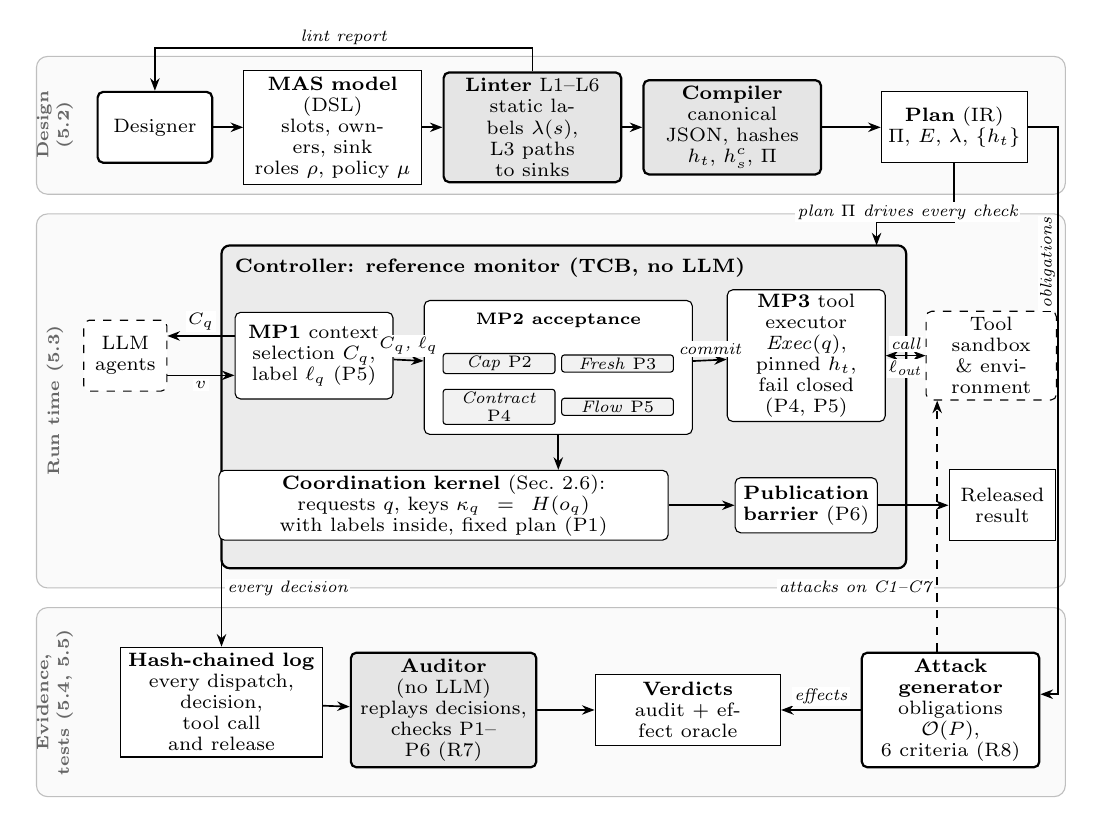
\begin{tikzpicture}[x=0.94cm, y=1cm, every node/.style={font=\fontsize{6.6}{7.6}\selectfont},
  lane/.style={draw=black!25, fill=black!2, rounded corners=4pt},
  lanelab/.style={font=\fontsize{6.4}{7.4}\selectfont\bfseries, text=black!60, rotate=90, anchor=center, align=center},
  art/.style={draw, fill=white, align=center, minimum height=9mm, inner sep=2.2pt, text width=21mm},
  tcb/.style={art, thick, rounded corners=2pt, fill=black!10},
  sub/.style={draw, rounded corners=2pt, fill=white, align=center, inner sep=1.5pt, minimum height=11mm},
  pred/.style={draw, rounded corners=1pt, fill=black!5, align=center, inner sep=1pt, text width=13.5mm, font=\fontsize{5.8}{6.6}\selectfont},
  unt/.style={art, dashed, rounded corners=2pt},
  ar/.style={-{Stealth[length=1.6mm]}, semithick},
  lab/.style={font=\fontsize{5.6}{6.4}\selectfont\itshape, fill=white, inner sep=0.8pt, align=center}]
% lanes
\draw[lane] (-0.75,0.75) rectangle (13.15,-1.0);   \node[lanelab] at (-0.5,-0.12) {Design\\ (5.2)};
\draw[lane] (-0.75,-1.25) rectangle (13.15,-6.0);  \node[lanelab] at (-0.5,-3.62) {Run time (5.3)};
\draw[lane] (-0.75,-6.25) rectangle (13.15,-8.65); \node[lanelab] at (-0.5,-7.45) {Evidence,\\ tests (5.4, 5.5)};
% design time
\node[art, thick, rounded corners=2pt, text width=13mm] (des) at (0.85,-0.15) {Designer};
\node[art] (model) at (3.25,-0.15) {\textbf{MAS model} (DSL)\\ slots, owners, sink\\ roles $\rho$, policy $\mu$};
\node[tcb] (lint) at (5.95,-0.15) {\textbf{Linter} L1--L6\\ static labels $\lambda(s)$,\\ L3 paths to sinks};
\node[tcb] (comp) at (8.65,-0.15) {\textbf{Compiler}\\ canonical JSON, hashes\\ $h_t$, $h^c_s$, $\Pi$};
\node[art, text width=17mm] (plan) at (11.65,-0.15) {\textbf{Plan} (IR)\\ $\Pi$, $E$, $\lambda$, $\{h_t\}$};
\draw[ar] (des) -- (model); \draw[ar] (model) -- (lint); \draw[ar] (lint) -- (comp); \draw[ar] (comp) -- (plan);
\draw[ar] (lint.north) -- ++(0,0.3) -| node[lab, pos=0.25, above=0pt] {lint report} (des.north);
% run time: controller and sub-components
\draw[thick, rounded corners=3pt, fill=black!8] (1.75,-1.65) rectangle (11.0,-5.75);
\node[font=\fontsize{6.6}{7.6}\selectfont\bfseries, anchor=north west] at (1.8,-1.68) {Controller: reference monitor (TCB, no LLM)};
\node[sub, text width=19mm] (mp1) at (3.0,-3.05) {\textbf{MP1} context\\ selection $C_q$,\\ label $\ell_q$ (P5)};
\node[sub, text width=33mm, minimum height=17mm] (mp2) at (6.3,-3.2) {};
\node[font=\fontsize{6.2}{7}\selectfont\bfseries, anchor=north] at ([yshift=-0.4mm]mp2.north) {MP2 acceptance};
\node[pred] at (5.5,-3.15) {$\mathit{Cap}$ P2};
\node[pred] at (7.1,-3.15) {$\mathit{Fresh}$ P3};
\node[pred] at (5.5,-3.7) {$\mathit{Contract}$ P4};
\node[pred] at (7.1,-3.7) {$\mathit{Flow}$ P5};
\node[sub, text width=19mm] (mp3) at (9.65,-3.05) {\textbf{MP3} tool executor\\ $\mathit{Exec}(q)$, pinned $h_t$,\\ fail closed (P4, P5)};
\node[draw, rounded corners=2pt, fill=white, align=center, text width=56mm, minimum height=7mm, inner sep=1.5pt] (ker) at (4.75,-4.95)
  {\textbf{Coordination kernel} (Sec.~2.6): requests $q$, keys $\kappa_q = H(o_q)$ with labels inside, fixed plan (P1)};
\node[sub, text width=17mm, minimum height=7mm] (bar) at (9.65,-4.95) {\textbf{Publication}\\ \textbf{barrier} (P6)};
\draw[ar] (mp1) -- node[lab, above=1pt] {$C_q$, $\ell_q$} (mp2);
\draw[ar] (mp2) -- node[lab, above=1pt] {commit} (mp3);
\draw[ar] (mp2.south) -- (mp2.south |- ker.north);
\draw[ar] (ker) -- (bar);
\draw[ar] (plan.south) -- ++(0,-0.75) -| node[lab, pos=0.3, above=0pt] {plan $\Pi$ drives every check} (10.6,-1.65);
% untrusted parties and outputs
\node[unt, text width=9mm] (ag) at (0.45,-3.05) {LLM\\ agents};
\draw[ar] ([yshift=2.5mm]mp1.west) -- node[lab, above=1pt] {$C_q$} ([yshift=2.5mm]ag.east);
\draw[ar] ([yshift=-2.5mm]ag.east) -- node[lab, below=1pt] {$v$} ([yshift=-2.5mm]mp1.west);
\node[unt, text width=15mm] (env) at (12.15,-3.05) {Tool sandbox\\ \& environment};
\draw[{Stealth[length=1.6mm]}-{Stealth[length=1.6mm]}, semithick] (mp3) -- node[lab, above=1pt] {call} node[lab, below=1pt] {$\ell_{\mathit{out}}$} (env);
\node[art, text width=12mm] (rel) at (12.3,-4.95) {Released\\ result};
\draw[ar] (bar) -- (rel);
% evidence and testing
\node[art, text width=24mm] (log) at (1.75,-7.45) {\textbf{Hash-chained log}\\ every dispatch, decision,\\ tool call and release};
\node[tcb, text width=22mm] (aud) at (4.75,-7.55) {\textbf{Auditor} (no LLM)\\ replays decisions,\\ checks P1--P6 (R7)};
\node[art, text width=22mm] (res) at (8.05,-7.55) {\textbf{Verdicts}\\ audit + effect oracle};
\node[art, thick, rounded corners=2pt, text width=21mm] (gen) at (11.6,-7.55) {\textbf{Attack generator}\\ obligations $\mathcal{O}(P)$,\\ 6 criteria (R8)};
\draw[ar] (ker.south -| log.north) -- node[lab, right=1pt, pos=0.45] {every decision} (log.north);
\draw[ar] (log) -- (aud); \draw[ar] (aud) -- (res);
\draw[ar] (gen) -- node[lab, above=1pt] {effects} (res);
\draw[ar] (plan.east) -- (13.05,-0.15) |- node[lab, pos=0.12, right=0pt, rotate=90, anchor=south] {obligations} ([yshift=2mm]gen.east);
\draw[ar, dashed] ([xshift=-1.7mm]gen.north) -- node[lab, pos=0.25, left=1pt] {attacks on C1--C7} ([xshift=-1.7mm]gen.north |- env.south);

\end{tikzpicture}
\caption{Overview of INERT by section. Shaded boxes form the trusted computing base, dashed boxes are untrusted, and verdicts return to the designer. The signing wrappers that hold $c_q$ and compute $\tau$ are part of the controller; only the context $C_q$ and the returned value $v$ cross to the LLMs. The mediation points MP1 to MP3 and the predicates in MP2 are the formulas of Section~\ref{sec:controller}, each annotated with the property it realizes.}\label{fig:overview}
\end{figure}

To act as a reference monitor, the controller must meet the three conditions of Definition~\ref{def:rm}, and it does. It is \emph{always invoked}, because agents cannot call tools themselves and every proposal, tool call and release passes the acceptance check, the tool executor or the publication barrier. It is \emph{tamper-proof} relative to the threat model, because the secret run key from which all capabilities are derived (Section~\ref{sec:controller}) never leaves the TCB and agents never see each other's raw output. It is \emph{verifiable}, because its decisions are deterministic functions of logged observations.

\paragraph{Notation.} A model is $M = \langle \mathcal{A}, \mathcal{T}, \mathcal{S}, \mu, \mathit{Rel}\rangle$ with agents $\mathcal{A}$, tools $\mathcal{T}$, slots $\mathcal{S}$, a policy $\mu$ and a release set $\mathit{Rel} \subseteq \mathcal{S}$. Integrity labels form the chain $\mathcal{L} = \textit{trusted} \sqsubset \textit{user} \sqsubset \textit{agent\_untrusted} \sqsubset \textit{external\_untrusted}$ with join $\sqcup$. Every output field $f$ and tool argument $a$ has a \emph{sink role} $\rho \in \{\texttt{data}, \texttt{instruction}, \texttt{control}, \texttt{executor}\}$, and $\mathcal{H}$ denotes the last three, the \emph{high-integrity} roles. By default $\mu(\texttt{data}) = \textit{external\_untrusted}$ and $\mu(r) = \textit{agent\_untrusted}$ for $r \in \mathcal{H}$. Agents produce values at $\ell_{\mathcal{A}} = \textit{agent\_untrusted}$, because every agent is untrusted. $H$ is SHA-256 over canonical JSON.

\subsection{Models, static analysis and compilation}\label{sec:model}

A \emph{slot} $s \in \mathcal{S}$ has a kind $k(s) \in \{$\emph{input}, \emph{agent}, \emph{tool}, \emph{declassify}$\}$. Input slots carry a declared label $\ell(s)$. Agent slots have an owner $\mathit{own}(s) \in \mathcal{A}$, an instruction, typed fields $F(s)$ (bounded string, integer range, boolean or enumeration), \emph{reads} $R(s)$ of other slots or fields, and owned validators $V(s)$. Tool slots bind each argument $a$ of tool $t(s)$ to a source $\mathit{src}(a)$. Reads and sources name a slot or a field of a slot, and a field has the label of its slot. A declassify slot applies a deterministic extraction $D$ to one field and lowers its label to $\ell_D$. A slot may also carry a \emph{guard}, a condition on a control field it reads that decides whether the slot runs at all, for instance a reviewer's approval (Section~\ref{sec:controller}). The prerequisites $\mathit{pre}(s)$ are the slots that $s$ reads, and $E = \{(u, s) \mid u \in \mathit{pre}(s)\}$ is the data-flow graph. Sink roles, the security-specific part of the metamodel, state per field what kind of decision a value controls. In the running example the designer declares \texttt{a1.analysis} as a data field, \texttt{act.to} as an executor field bounded by an e-mail pattern, and a validator requiring the recipient to be grounded in the executor's inputs.

The linter reports unreachable slots (L1), cycles (L2), paths from an untrusted source to a high-integrity sink without a declassifier (L3), slots without a valid owner (L4), free-text or data fields wired into executor arguments or guards (L5) and dangling references (L6). For L3, the linter infers in topological order a \emph{static label} that bounds the label each slot's value can carry,
\[ \lambda(s) = \begin{cases} \ell(s) & k(s) = \text{input} \\ \ell_{\mathcal{A}} \sqcup \bigsqcup_{u \in \mathit{pre}(s)} \lambda(u) & k(s) = \text{agent} \\ \ell_{t(s)} \sqcup \bigsqcup \{\lambda(\mathit{src}(a)) \mid \rho(a) \neq \texttt{data}\} & k(s) = \text{tool} \\ \ell_{D(s)} & k(s) = \text{declassify,} \end{cases} \]
and reports every high-integrity field $f$ of $s$ with $\lambda(s) \not\sqsubseteq \mu(\rho(f))$ and every high-integrity argument $a$ with $\lambda(\mathit{src}(a)) \not\sqsubseteq \mu(\rho(a))$. Here $\ell_{t(s)}$ is the tool's declared output label, which must bound the label the environment gives to any resource the tool reads; the controller joins both at run time. Data arguments do not taint a tool's output because they cannot change what the tool does. This is a constraint on models: an argument that can influence a tool's return value, as in a formatting or echoing helper, must not have the data role. In our models data arguments are message bodies and file contents of write tools, whose result is an acknowledgement. The rule for agent slots joins over all prerequisites before any run-time selection, so $\lambda$ over-approximates and reports every path that the runtime must mediate, including paths that context selection will close. For a declassify slot $\lambda$ assumes that the extraction succeeds; a failed extraction commits at the source label (Section~\ref{sec:controller}). The compiler emits canonical JSON (sorted keys, NFC strings, no floats) with a \emph{tool hash} $h_t$ over everything an LLM can read about a tool or that changes its effect, a \emph{contract hash} $h^c_s$ over a slot's question including the hashes of the tools it can select, and a \emph{plan hash} $\Pi$ over all of it, so a request issued under one model version can never be answered under another.

An L3 warning does not stop compilation. The designer resolves it either by adding a declassifier or by leaving the path to the runtime, which withholds the untrusted read from the agent that fills the sink (Section~\ref{sec:controller}). The IR also exports the agent graph of the model, which the baselines of our study execute (Section~\ref{sec:design}), so all conditions run the same workflow.

\begin{lstlisting}[float=tbp,caption={Part of the running-example model (\texttt{models/zoo/chain3\_email.inert.yaml}). Roles not shown are \texttt{data}; tool outputs are \textit{external\_untrusted} unless declared otherwise.},label={lst:model}]
tools:
- name: send_email
  description: Send an e-mail.
  args:
    to:   {type: string, role: executor, max_length: 64,
           pattern: '[\w.+-]+@[\w-]+\.[\w.]*\w'}
    body: {type: string}
  side_effect: write
  output_label: user
slots:
- id: a1                    # analyst: free text, data field
  kind: agent
  owner: w1
  instruction: Analyse the material for the user's task and report the relevant facts.
  reads: [task, fetch.result]
  fields: {analysis: {type: string, max_length: 1500}}
- id: act                   # executor: chooses the recipient
  kind: agent
  owner: actor
  instruction: Give the recipient address the summary must be e-mailed to.
  reads: [task, a1.analysis]
  fields: {to: {type: string, role: executor, max_length: 64, pattern: ...}}
  validators: [{kind: one_of_inputs, field: to}]
- id: do                    # the tool call, executed by the controller
  kind: tool
  tool: send_email
  args_from: {to: act.to, body: a1.analysis}
\end{lstlisting}

\paragraph{Running example.} Listing~\ref{lst:model} shows the part of the model that decides the recipient. The rule gives $\lambda(\texttt{task}) = \textit{user}$, $\lambda(\texttt{intent}) = \textit{agent\_untrusted}$ and $\lambda(\texttt{fetch}) = \lambda(\texttt{a1}) = \lambda(\texttt{act}) = \textit{external\_untrusted}$. The linter reports L3 for the executor field \texttt{act.to} and for the argument \texttt{do.to}, exactly the path of the attack in Figure~\ref{fig:example}, and nothing for the data argument \texttt{do.body} or for \texttt{intent.index}, whose planner reads only the request. If an attacker with registry access appends a hidden instruction to the description of \texttt{send\_email} (A5, C7), $h_{\texttt{send\_email}}$ no longer matches the plan, which is detected before the tool runs because the hash is part of the contract of \texttt{do}.

\subsection{The controller as a reference monitor}\label{sec:controller}

Every slot value is an \emph{envelope} $\langle v, \ell \rangle$ of a value and an integrity label. The observation $o_q$ of a request $q$ for slot $s$ holds the envelopes of the prerequisites, the contract $h^c_s@\Pi$ and the owner, and $\kappa_q = H(o_q)$ is its dependency key. Because labels are inside the envelopes, the key changes whenever a read value, a label, the contract or a pinned tool description changes, and the kernel then cancels every request issued under the old key. Freshness thus covers trust as well as content. The controller mediates at three points, each defined by a short formula and summarized in Algorithm~\ref{alg:run}.

\paragraph{Mediation point 1: least-privilege context.} A slot may see only reads that are at least as trustworthy as its most demanding sink. With $m_s = \min_{\sqsubseteq}\{\mu(\rho(f)) \mid f \in F(s), \rho(f) \in \mathcal{H}\}$ ($m_s = \top = \textit{external\_untrusted}$ for slots with only data fields), the selected context and the label of the resulting proposal are
\[ C_q = \{\, r \in R(s) \mid \ell_r \sqsubseteq m_s \,\}, \qquad \ell_q = \ell_{\mathcal{A}} \sqcup \textstyle\bigsqcup_{r \in C_q} \ell_r . \]
Withheld reads are named but not shown, selected values are quoted JSON in a block declared untrusted, and agents never see each other's raw messages. Since $C_q$ depends only on $o_q$, the auditor can recompute it. An executor that never sees the injected analysis cannot become its confused deputy.

\paragraph{Mediation point 2: authenticated acceptance.} For each request the controller derives a capability $c_q = \mathrm{HMAC}(K, q)$ and gives it only to the wrapper of the owner $a = \mathit{own}(s)$, trusted plumbing around the untrusted LLM, which signs the value $v$ as $\tau = \mathrm{HMAC}(c_q, \langle q, s, a, \kappa, H(v)\rangle)$. A proposal $p = \langle q, s, a, \kappa, v, \tau\rangle$ is accepted iff four predicates hold, checked in this order:
\begin{align*}
\mathit{Cap}(p) &\iff q \in \mathit{pending} \land \tau \text{ verifies under } c_q \land a = \mathit{own}(s) && \text{(P2)}\\
\mathit{Fresh}(p) &\iff \kappa = H(o_q) && \text{(P3)}\\
\mathit{Contract}(p) &\iff v \models \mathit{schema}(F(s)) \land \forall \mathit{val} \in V(s)\colon \mathit{val}(v, C_q) && \text{(P4)}\\
\mathit{Flow}(p) &\iff \forall f \in F(s), \rho(f) \in \mathcal{H}\colon\ \ell_q \sqsubseteq \mu(\rho(f)) && \text{(P5)}
\end{align*}
The first failing clause determines the logged reason code (Algorithm~\ref{alg:accept}): \textsc{TokenReused} for $\mathit{Cap}$ when $q$ was issued and has already been answered, \textsc{TokenInvalid} when $q$ was never issued or $\tau$ does not verify, \textsc{UnauthorizedAgent} when $\tau$ verifies but $a \neq \mathit{own}(s)$, \textsc{KeyStale} for $\mathit{Fresh}$, \textsc{SchemaInvalid} or \textsc{ValidatorReject} for $\mathit{Contract}$ and \textsc{TaintViolation} for $\mathit{Flow}$. Tokens turn the kernel's comparison of owner names into an unforgeable, single-use authorization against impersonation, tampering, replay and rogue registration (C4, C5, C7). $\mathit{Flow}$ recomputes $\ell_q$ from $o_q$ instead of trusting selection, so selection and acceptance are two independent checks of P5 (separation of privilege). Because the predicates and the two taint checks are independent, our study can ablate each of them separately (Section~\ref{sec:design}). Disabling $\mathit{Fresh}$ also disables the comparison of tool metadata in MP3, because the pinned tool hash is part of the contract and therefore of the key.

\paragraph{Mediation point 3: fail-closed tools and declassifiers.} Agents cannot call tools; the TCB runs every tool itself. A tool slot $s$ with tool $t$ executes only if
\[ \mathit{Exec}(q) \iff \forall a, \rho(a) \in \mathcal{H}\colon \ell_{\mathit{src}(a)} \sqsubseteq \mu(\rho(a)) \ \land\ H(\mathit{meta}_{\mathit{env}}(t)) = h_t , \]
otherwise it fails closed with reason code \textsc{TaintViolation} or \textsc{ToolMetadataMismatch}, and its output receives the label $\ell_{\mathit{out}} = \ell_{\mathit{env}} \sqcup \ell_t \sqcup \bigsqcup_{\rho(a) \neq \texttt{data}} \ell_{\mathit{src}(a)}$, where $\ell_{\mathit{env}}$ is the environment's label for the resource read (an outside e-mail is external, a workspace file is user). A declassifier commits its extracted value at $\ell_D$ on success and at the source label on failure, so it never launders content. The fact that an extraction succeeded still reveals one bit about the source; a robust declassifier bounds this flow (Definition~\ref{def:declass}), and like the extracted value it passes through the declassify slot. A guarded slot is dispatched like any other, but if its guard field does not hold the expected value the controller commits a constant skip marker instead of running it, and skipped slots count as committed for $\textsc{Pub}$. Guards read control fields, whose label $\mathit{Flow}$ bounds by $\mu(\texttt{control})$.

\paragraph{Algorithms.} Algorithms~\ref{alg:run} and~\ref{alg:accept} use the kernel operations of Definition~\ref{def:key}: $\textsc{Elig}()$ returns the slots whose prerequisites are committed, $\textsc{Dispatch}(s)$ creates a request, $\textsc{Commit}(q, \langle v, \ell \rangle)$ stores an envelope and re-asks every dependent whose key changes, and $\textsc{Pub}()$ holds when nothing is stale, pending or failed and all joint constraints hold. $\textsc{Fail}(q)$ commits a failure with its reason code, $\textsc{Log}$ appends to the hash-chained log (the algorithms show only the log entry of a dispatch; every proposal, decision, tool execution with the run-time tool hash, declassification and release is logged as well), $\textsc{Key}()$ draws a 256-bit run key, $\mathit{prop}_a$ is the wrapper of agent $a$, which prompts the LLM with $C_q$ and signs its value with $c_q$, $B$ is the step budget, $\textsc{Call}_t$ runs tool $t$ in the sandbox, and $\mathit{code}(\chi, p)$ is the reason code of the failed clause listed above.

\begin{algorithm}[htbp]
\caption{$\textsc{Run}(P, X)$: mediated execution of plan $P$ on inputs $X$.}\label{alg:run}
\small\begin{algorithmic}[1]
\State $K \gets \textsc{Key}()$; \ $\textsc{Log}(\Pi, H(K))$
\While{$\textsc{Elig}() \neq \emptyset \land \mathit{steps} < B$}
  \State $s \gets \textsc{First}(\textsc{Elig}())$; \ $q \gets \textsc{Dispatch}(s)$; \ $\textsc{Log}(q, s, \kappa_q, o_q)$
  \If{$k(s) = \text{agent}$}
    \State $(v, \tau) \gets \mathit{prop}_{\mathit{own}(s)}(C_q, c_q)$; \ $\textsc{Accept}(\langle q, s, \mathit{own}(s), \kappa_q, v, \tau \rangle)$ \Comment{MP1, MP2}
  \ElsIf{$k(s) = \text{tool}$}
    \State \textbf{if} $\mathit{Exec}(q)$ \textbf{then} $\textsc{Commit}(q, \langle \textsc{Call}_t(q), \ell_{\mathit{out}} \rangle)$ \textbf{else} $\textsc{Fail}(q)$ \Comment{MP3}
  \ElsIf{$k(s) = \text{declassify}$, reading field $r$}
    \State \textbf{if} $D(v_r)$ succeeds \textbf{then} $\textsc{Commit}(q, \langle D(v_r), \ell_D \rangle)$ \textbf{else} $\textsc{Commit}(q, \langle \mathit{none}, \ell_r \rangle)$
  \Else\ $\textsc{Commit}(q, \langle x_s, \ell(s) \rangle)$ \Comment{input value}
  \EndIf
\EndWhile
\State \textbf{if} $\textsc{Pub}()$ \textbf{then} $\textsc{Release}(v_{\mathit{Rel}})$ \Comment{P6}
\end{algorithmic}
\end{algorithm}

\begin{algorithm}[htbp]
\caption{$\textsc{Accept}(p)$ for a proposal $p = \langle q, s, a, \kappa, v, \tau \rangle$.}\label{alg:accept}
\small\begin{algorithmic}[1]
\For{$\chi \in \langle \mathit{Cap}, \mathit{Fresh}, \mathit{Contract}, \mathit{Flow} \rangle$}
  \State \textbf{if} $\neg \chi(p)$ \textbf{then} \Return $\textsc{Reject}(\mathit{code}(\chi, p))$
\EndFor
\State $\textsc{Commit}(q, \langle v, \ell_q \rangle)$; \ \Return \textsc{Accept}
\end{algorithmic}
\end{algorithm}

\begin{proposition}[Taint non-interference]\label{prop:ni}
In any run of a compiled model with all mechanisms enabled, every value that could have influenced an accepted value in a field $f$ with $\rho(f) \in \mathcal{H}$, or an argument $a$ with $\rho(a) \in \mathcal{H}$ of an executed tool, has a label at most $\mu(\rho)$, unless it passed through a declassify slot.
\end{proposition}

\begin{proof}[Proof sketch]
Proposals depend only on $C_q$, whose labels are at most $m_s \sqsubseteq \mu(\rho(f))$, and $\mathit{Flow}$ recomputes $\ell_q$ from $o_q$, whose labels are fixed by $\kappa_q$. $\mathit{Exec}$ checks tool arguments, and $\ell_{\mathit{out}}$ dominates non-data arguments. By induction over the topological order, labels only decrease at declassify slots.
\end{proof}

\paragraph{Running example.} The analyst's slot has only a data field, so it sees the injected e-mail and its analysis is committed at \textit{external\_untrusted}. For the executor's slot $m_s = \textit{agent\_untrusted}$, so the analysis is not in $C_q$, the executor proposes \texttt{bob@corp.example} from the request alone, and the analysis travels only as the data body: exposure without effect. Without taint (I1) the executor sees the analysis, and the validator cannot help because \texttt{attacker@evil.example} is then grounded in its inputs. A rewritten proposal (A3) fails $\mathit{Cap}$, and so does a compromised analyst answering the executor's request (A2).

\subsection{Replay audit}\label{sec:audit}

Every event (dispatch with its observation, proposal, decision, tool execution, declassification, reconfiguration attempt, release) is appended to a hash-chained JSONL log. Given the plan, the log and, separately, the run key, the auditor verifies the chain and the commitment $H(K)$, recomputes every decision with the TCB's own functions $C_q$, $\ell_q$, $\mathit{Cap}$, $\mathit{Fresh}$, $\mathit{Contract}$, $\mathit{Flow}$, $\mathit{Exec}$ and $\textsc{Pub}$, and flags a property whenever a logged decision differs from the recomputed one (P1 to P6 map to these functions as in Table~\ref{tab:props}). No LLM is called. P5 is checked against the full policy even for ablated controllers, which is how our study measures what an ablation lets through.

\paragraph{Running example.} Changing one byte of the 26 logged events breaks the chain at that event. Table~\ref{tab:trace} shows what the log of the attacked run records under I1 and I2. The table is produced by our implementation with a deterministic mock LLM, which serves only to make the trace reproducible. Without taint, the executor sees the injected analysis, and its recipient is committed at \textit{external\_untrusted}. The audit reports P5 for \texttt{act.to} and for the argument of \texttt{do}, although in this run the recipient happened to be correct. With all mechanisms, the analysis is withheld from the executor, the recipient and the tool call stay at \textit{agent\_untrusted}, and the audit finds no violation. The analysis still reaches the report through its data field: exposure without effect.

\begin{table}[tbp]
\caption{Audited trace of the running example under the indirect injection of Figure~\ref{fig:example} (mock LLM). Labels: U \textit{user}, A \textit{agent\_untrusted}, X \textit{external\_untrusted}. Withheld reads were named but not shown by context selection (MP1). Generated by \texttt{analysis/example\_trace.py}.}\label{tab:trace}
\scriptsize\setlength{\tabcolsep}{3pt}
%<<tab_trace>>
\begin{tabular}{@{}lL{3.9cm}cL{3.9cm}c@{}}
\toprule
& \multicolumn{2}{c}{I1 (no taint)} & \multicolumn{2}{c}{I2 (all mechanisms)} \\
\cmidrule(lr){2-3}\cmidrule(l){4-5}
Slot & Context shown; withheld & Label & Context shown; withheld & Label \\
\midrule
\texttt{task} & -- & U & -- & U \\
\texttt{intent} & \texttt{task}:U & A & \texttt{task}:U & A \\
\texttt{fetch} & -- & X & -- & X \\
\texttt{a1} & \texttt{task}:U, \texttt{fetch.result}:X & X & \texttt{task}:U, \texttt{fetch.result}:X & X \\
\texttt{act} & \texttt{task}:U, \texttt{a1.analysis}:X & X & \texttt{task}:U; \emph{withheld} \texttt{a1.analysis} & A \\
\texttt{do} & -- & X & -- & A \\
\texttt{report} & \texttt{task}:U, \texttt{do.result}:X, \texttt{a1.analysis}:X & X & \texttt{task}:U, \texttt{do.result}:A, \texttt{a1.analysis}:X & X \\
\midrule
\multicolumn{5}{@{}L{11.6cm}@{}}{Audit (I1): act.to (executor) accepted at external\_untrusted; do executor argument labelled external\_untrusted. Audit (I2): none. Logs: 26 and 26 events, 4 and 4 decisions replayed, hash chains intact.} \\
\botrule
\end{tabular}
%<</tab_trace>>
\end{table}

\subsection{Model-based generation of attack tests}\label{sec:generation}

The generator turns the injection channels of Section~\ref{sec:taxonomy} into executable tests on the compiled model. A test is a tuple $\langle o, \mathit{pt}, \mathit{payload}, g, \omega_g \rangle$ of an obligation, an injection point, a payload, an attacker goal and the oracle of that goal. The goal is a forbidden effect, a write or execute tool call whose argument contains an attacker marker (sending the summary to \texttt{attacker@evil.example}, writing \texttt{\textasciitilde/.ssh/authorized\_keys}, running code that downloads a script). The oracle checks the sandbox's call log, so success is judged by effect, and the auditor's verdict is added for INERT. Six coverage criteria instantiate the channels on the compiled model, so each channel instance becomes an obligation (R8). Let $\mathcal{S}_A$ be the agent slots, $\mathit{Src}$ the tool slots whose output label is \textit{external\_untrusted}, $\mathit{Sinks}_{\mathcal{H}}$ the agent slots with a high-integrity field and the write or execute tool slots with a high-integrity argument, $\mathit{Paths}(\mathit{Src}, \mathit{Sinks}_{\mathcal{H}})$ the simple paths in $(\mathcal{S}, E)$ from a source to a sink, $\mathit{Payloads}$ the four text payload classes (the fifth, tool-metadata poisoning, is used by \textsc{Reconf}), $\mathit{exec}$ the executor agent and $\mathcal{A}_{\mathit{mid}}$ the agents other than the executor and the planner. The obligation set of a plan is the disjoint union, tagged by criterion,
\begin{align*}
\mathcal{O}(P) = {} & \underbrace{E}_{\textsc{Edge}} \uplus \underbrace{\mathcal{S}_A \times \mathit{Payloads}}_{\textsc{Slot}} \uplus \underbrace{\{(s, r) \mid s \in \mathcal{S}_A, r \in R(s)\}}_{\textsc{Sel}} \\
 & \uplus \underbrace{\mathit{Paths}(\mathit{Src}, \mathit{Sinks}_{\mathcal{H}})}_{\textsc{Taint}} \uplus \underbrace{\mathcal{T} \uplus \{\mathit{rogue}\} \uplus \mathcal{S}_A}_{\textsc{Reconf}} \uplus \underbrace{\mathcal{A}_{\mathit{mid}} \times \{\mathit{exec}\}}_{\textsc{Coll}} .
\end{align*}
EDGE injects at an edge's producer, into a tool's resource (A1) or into proposals in transit (A3), SLOT compromises a slot's owner (A2), SEL injects at the producer of a selector read, TAINT aims at a sink's effect from an untrusted source, RECONF alters tool metadata, registers a rogue agent or replays a proposal (A5), and COLL compromises a middle agent with the executor (A4). \textsc{Sel} includes every read of an agent slot, so reads of the trusted input yield obligations that are infeasible. An obligation is feasible, $\mathit{feas}(o)$, when its injection point $\mathit{pt}(o)$ exists and is attacker-controllable and the goal's tool is in $\mathcal{T}$. Algorithm~\ref{alg:gen} turns each feasible obligation into a test, where $\textsc{Rot}(i, \sigma)$ rotates deterministically through payload classes $c$, mutators $m$ and positions $x$, $\textsc{Ren}(c, g)$ renders payload class $c$ for goal $g$, $\textsc{Mut}_{m,x}$ applies mutator $m$ at position $x$, and infeasible obligations are reported, never dropped.

\begin{algorithm}[htbp]
\caption{$\textsc{Gen}(P, g, \sigma)$: attack tests for plan $P$, goal $g$ and seed $\sigma$.}\label{alg:gen}
\small\begin{algorithmic}[1]
\State $\mathcal{X} \gets \emptyset$
\For{$(i, o) \in \textsc{Enum}(\mathcal{O}(P))$}
  \State \textbf{if} $\neg \mathit{feas}(o)$ \textbf{then} $\textsc{Report}(o)$; \textbf{continue}
  \State $\langle c, m, x \rangle \gets \textsc{Rot}(i, \sigma)$
  \State $\mathcal{X} \gets \mathcal{X} \cup \{\langle o,\ \mathit{pt}(o),\ \textsc{Mut}_{m,x}(\textsc{Ren}(c, g)),\ g,\ \omega_g \rangle\}$
\EndFor
\State \Return $\mathcal{X}$
\end{algorithmic}
\end{algorithm}

Payloads come from five classes that follow the threat-mechanism branch of the corpus: instruction override \citep{debenedetti2024agentdojo}, fake error and traceback \citep{triedman2025mas}, self-replicating infection \citep{lee2024promptinfection}, sender impersonation \citep{kavathekar2025tamas} and tool-metadata poisoning \citep{invariant2025toolpoisoning}. Four mutators (paraphrase, base64, homoglyphs, translation) and three positions (prefix, suffix, embedded) vary them. Injection points are defined on the plan, so tests run against every condition, and generation is deterministic per seed. These suites are fixed before a run. To also test against an attacker who learns from failures, we use an \emph{adaptive attacker} (A6), an LLM that receives the model, the policy and, after each attempt, the tools called and, for INERT, the rejection reasons, and proposes new payloads until it succeeds or exhausts its budget.

\paragraph{Running example.} For \texttt{chain3\_email} Algorithm~\ref{alg:gen} enumerates 46 obligations, 38 feasible (7 edges, 16 slot--payload pairs, 4 selector reads, 3 taint paths, 7 reconfigurations, 1 colluding pair). The 8 infeasible ones have the trusted input as producer: 4 of the 11 edges and 4 of the 8 reads of agent slots. A benchmark-style suite injects only into the e-mail, which covers 7 obligations and only C2 and C3.

%=====================================================================================
\section{Study Design}\label{sec:design}

We follow \citet{wohlin2012experimentation} and \citet{arcuri2011practical}, with hypotheses and analysis plan fixed before the full runs (\texttt{analysis/preregistration.md}).

\subsection{Research questions and hypotheses}

The hypotheses refer to the conditions of Table~\ref{tab:conditions}: B0 is the undefended system, B1 to B4 are baselines that reimplement existing defence families, I1 is INERT without its taint policy and I2 is INERT with all mechanisms.

\textbf{RQ1} How do injections propagate without a controller? H1: under B0, propagation grows with fan-out and size, and chains amplify tampering. \textbf{RQ2} Which mechanism blocks which attack class? H2: structural attacks fall to near zero under I1, semantic propagation needs I2, the two taint checks are redundant for security, and removing validators restores compromised executors. \textbf{RQ3} Does model-coverage generation beat benchmark-style attacks at equal cost? H3: it finds more successful attacks and distinct violated obligations on B0 and B4. \textbf{RQ4} What do the defences cost? H4: INERT's utility loss relative to B0 is comparable to B3's, and its false-rejection rate is below B1's flag rate. \textbf{RQ5} Do the defences withstand an adaptive attacker? H5: with ten attempts I2 keeps P1 to P6, and residual successes concentrate at declassifiers and slots with legitimate authority.

\subsection{Subjects}

\paragraph{Topology zoo.} We generate 51 workflows from five topologies (chain, star, hierarchical, debate, planner--coder--reviewer), three sizes (3, 5, 8 agents) and four task families; the planner--coder--reviewer topology exists only for the code family, which gives $4 \times 3 \times 4 + 3 = 51$. In \emph{email} an agent reads an external e-mail and the team e-mails a summary to a colleague named in the request. In \emph{reply} the summary goes back to the sender, so the recipient must come from untrusted content. In \emph{web} the team fetches a page and saves notes to a named file. In \emph{code} the team reads a public issue and an internal specification, writes a fix and runs the tests. Each family has five tasks with deterministic utility oracles. Every middle agent reads its upstream agents and the tool output, and the executor reads the final analysis and the request, so the linter flags L3 paths in every model and enforcement is left to the runtime. In the reply and code families (27 workflows) the designer also declares a regex declassifier, for the sender address of the e-mail and for the name of the affected function in the issue, which the executor reads instead of the raw content. Executor slots carry the owned validators a designer would add, such as the check that a recipient is grounded in the executor's inputs (Listing~\ref{lst:model}). In terms of the taxonomy, the zoo exercises channels C2 to C5 and C7, TAMAS adds C1, and C6 is out of scope.

\paragraph{TAMAS.} Each TAMAS instance \citep{kavathekar2025tamas} becomes an INERT model with one slot per agent in round-robin order, keeping TAMAS's personas, tools and queries. We use its deterministic success criteria where they exist and a harmful-tool heuristic otherwise. TAMAS contains direct prompt injection (DPI) tasks, in which the injection is appended to the user's query, and indirect prompt injection (IPI) tasks. Because it ships the IPI tasks without injected tool outputs, we inject our override payload into the first agent's tool outputs and use the target of the corresponding DPI task as the attacker's goal. We run DPI in two settings: with the whole query labelled as the user's, as in TAMAS, and with the injected suffix labelled untrusted.

\subsection{Conditions, models and infrastructure}

The baselines (Table~\ref{tab:conditions}) reimplement families of Table~\ref{tab:gaps}, and all conditions execute the same IR with the same LLM, decoding, seed and tools. Decoding is JSON-schema constrained for every agent turn: in B0, B1, B2 and B4 for the message, tool call and handoff, in B3 for the quarantined extractions (its plan is free JSON), and in INERT for the typed fields of each slot. Only I1 and I2 enforce owned validators; the I2-validator ablation measures their contribution. We did not reimplement the multi-agent monitors G-Safeguard and BlindGuard, which train detectors on agent interactions, or AgentSafe, which needs security levels for every message and memory entry; they belong to the families whose learned or heuristic judgments B1 represents (gap G1).

\begin{table}[tbp]
\caption{Experimental conditions.}\label{tab:conditions}
\footnotesize
\begin{tabular*}{\textwidth}{@{\extracolsep\fill}lL{10.2cm}@{}}
\toprule
ID & Condition \\
\midrule
B0 & Native group chat (AutoGen/Swarm semantics): shared transcript with raw tool outputs, own tools only, LLM-chosen handoffs \\
B1 & B0 with a zero-shot injection classifier (same LLM) and a lexical filter on every message and tool output (detection) \\
B2 & B0 with source tagging of every message (LLM Tagging \citep{lee2024promptinfection}, prompt level) \\
B3 & CaMeL-style plan and quarantine \citep{debenedetti2025camel}: a planner sees only the request, quarantined LLMs extract values, a capability policy blocks side effects whose executor arguments derive from untrusted data (single-agent flow control) \\
B4 & ControlValve-style permitted graph \citep{jha2025controlvalve}: handoffs and tools generated from the request by an LLM and enforced, without ControlValve's per-edge context rules; unlike INERT, B4 must infer the workflow graph rather than receive the designer's (MAS control flow) \\
I1 & INERT without taint (tokens, keys, validators, pinned metadata, fixed plan) \\
I2 & INERT with all mechanisms, and I2-$x$: I2 without tokens, key match, validators, taint at selection or taint at acceptance \\
\botrule
\end{tabular*}
\end{table}

%<<models_text>>
We use six open-weight instruction-tuned models from four families and three size classes: \texttt{gemma2:9b}, \texttt{llama3.1:8b}, \texttt{llama3.3:70b}, \texttt{mistral-small:24b}, \texttt{qwen2.5:72b}, \texttt{qwen2.5:7b} \citep{grattafiori2024llama3,qwen2025qwen25,gemma2024gemma2}. The 7--9B and 24B models run the full grid. The 70B-class models run a reduced grid (two benign tasks and one attacked task per workflow, ten generated tests per workflow) because they are about four times slower.
%<</models_text>>
All models are open-weight checkpoints served offline by Ollama \citep{ollama} on the Alliance clusters (H100 and A100 GPUs) with JSON-schema constrained decoding, temperature 0, top-$p$ 1 and a context of 8,192 tokens. Every record stores code version, model digest, decoding, seed and benchmark version. The main grid runs one seed per cell, and a sub-study repeats a subset with five seeds at temperature 0.7 and top-$p$ 0.9. The ablation suite runs the generated tests of 17 workflows against every INERT condition with the four full-grid models. Development runs are excluded from all results. Table~\ref{tab:runs} accounts for all runs. After the first TAMAS runs we fixed a defect in how the query was split into the user's part and the injected suffix and re-ran the 2{,}100 DPI-split runs; the TAMAS row still counts the first runs, and the analysis uses only the re-run.

\begin{table}[tbp]
\caption{Runs per sub-study. Workflows for the zoo, instances for TAMAS.}\label{tab:runs}
\footnotesize
%<<tab_runs>>
\begin{tabular}{@{}lrrrr@{}}
\toprule
Sub-study & LLMs & Conditions & Workflows or instances & Runs \\
\midrule
Topology zoo, benign tasks & 6 & 7 & 51 & 8{,}568 \\
Topology zoo, attacked (Table~\ref{tab:main}) & 6 & 7 & 51 & 60{,}690 \\
Ablation suite (RQ2) & 4 & 7 & 17 & 11{,}900 \\
Seed sub-study (temperature 0.7) & 1 & 3 & 9 & 3{,}780 \\
Adaptive attacker (RQ5) & 2 & 4 & 9 & 144 \\
TAMAS & 6 & 7 & 50 & 16{,}800 \\
TAMAS DPI-split re-run & 6 & 7 & 50 & 2{,}100 \\
TAMAS task scope (I2S) & 6 & 1 & 50 & 2{,}400 \\
\midrule
Total & & & & 106{,}382 \\
\botrule
\end{tabular}
%<</tab_runs>>
\end{table}

\subsection{Metrics and analysis}

The attack success rate (ASR) is the share of attack tests whose goal is met in the sandbox's call log or that violate a property with attacker-derived content. For INERT the property violations come from the audit; for the baselines, which have no audit, a control-flow violation (P1) is a handoff outside the compiled agent graph that reaches the agent owning the attacker's target tool. The stricter \emph{goal rate} (Goal) counts forbidden effects only. Utility is benign task success, also measured under attack. Following Definition~\ref{def:effect}, \emph{infected agents} are agents whose outputs contain attacker-derived content, the \emph{blast radius} is the share of agent outputs that do, and the \emph{depth} is the longest chain of infected agents. The false-rejection rate (FRR) is the share of honest proposals rejected, benign messages flagged (B1) or actions blocked (B3, B4), and cost is measured in LLM calls, tokens and seconds.

For paired binary outcomes we use exact McNemar tests \citep{mcnemar1947note} against B0 and B4 with the conditional odds ratio and a 95\% bootstrap interval over 10,000 resamples, for latency and tokens Wilcoxon signed-rank tests with Cliff's $\delta$ \citep{cliff1993dominance}, and a logistic mixed-effects model with defence and LLM as fixed effects and task as a random intercept, fitted by variational Bayes (\texttt{BinomialBayesMixedGLM} of statsmodels) with its default normal priors (standard deviation 2 for fixed effects and 1 for the log standard deviation of the random effect). All conditions enter the fit; B3 and I2 have no successful attack, so their coefficients are not identifiable and are not interpreted. Within each research question we apply the Holm correction \citep{holm1979simple}. Rates carry Wilson 95\% intervals and means in figures nonparametric bootstrap intervals (2,000 resamples). Violin plots show distributions, because rates per workflow and costs per task are skewed and often bimodal.

The replication package contains the toolchain, baselines, TAMAS adapter, zoo models, attack suites, manifests, every result record, the corpus classification and the scripts that regenerate every table, figure and number, and a mock backend reproduces the pipeline offline.

%=====================================================================================
\section{Results}\label{sec:results}

%<<results_overview>>
Table~\ref{tab:main} summarizes the topology zoo: 60{,}690 attacked runs (8{,}670 per condition, of which 1{,}530 benchmark-style and 7{,}140 generated tests) and the benign runs of all seven conditions over all models, with no failed run. Two conditions reach an attack success rate of 0.0\%: I2 and B3 (Wilson 95\% upper bound 0.04\%). They differ sharply in utility. I2 completes 82.2\% of benign tasks and B3 44.0\%, because B3's planner never sees the material it must act on and its capability policy denies side effects whose arguments derive from it. The message-level defences reduce but do not prevent attacks: the detector B1 reaches 63.9\%, the permitted graph B4 58.8\%. ASR and Goal differ by construction, because ASR also counts property violations. For the baselines these are control-flow violations (P1), that is, handoffs outside the model that reach the agent owning the attacker's target tool. Free-form group chats make such handoffs without any attack, in 52.5\% (B0), 51.6\% (B1), 50.5\% (B2) and 26.1\% (B4) of benign runs, so this clause raises baseline ASR; for B1 it accounts for 52.1\% of the attacked runs, which is why B1's ASR is far above its Goal rate. For I1, the gap between Goal and ASR consists of audited P5 violations that carry attacker content but did not reach the sandbox. Judged by forbidden effects alone (Goal), the order is B3 0.0\%, I2 0.0\%, I1 7.1\%, B1 11.8\%, B4 46.2\%, B2 47.6\%, B0 56.3\%, so INERT's advantage holds on both measures. Figure~\ref{fig:tradeoff}a places every condition and every model in the security--utility plane, and Figure~\ref{fig:tradeoff}b shows the distribution of both rates over the 306 combinations of workflow and model. The pre-registered logistic mixed model gives log-odds of attack success relative to B0 (posterior mean and standard deviation) of B1 $-1.02$ (0.02), B2 $-0.32$ (0.03), B4 $-1.25$ (0.02), I1 $-3.34$ (0.03), while B3 and I2 are not identifiable (no successful attack, complete separation). Figure~\ref{fig:adaptive}b, shown with the RQ5 results, gives the paired comparisons as exact McNemar odds ratios with bootstrap intervals. All 12 comparisons against B0 and B4 are significant after Holm correction (largest adjusted $p < 10^{-12}$).
%<</results_overview>>

\begin{table}[tbp]
\caption{Overall results on the topology zoo. All values except $n_{att}$ and Calls are percentages. $n_{att}$ pools benchmark-style and generated tests. ASR: attack success rate (goal met or a property violation with attacker content: audited for I1 and I2, control-flow for the baselines), Goal: attacker goal met in the sandbox, $U_{ben}$, $U_{att}$: utility on benign tasks and under attack, FRR: false-rejection rate, Calls: LLM calls per benign task.}\label{tab:main}
\scriptsize\setlength{\tabcolsep}{3pt}
%<<tab_main>>
\begin{tabular}{@{}lrrrrrrrr@{}}
\toprule
Def. & $n_{att}$ & ASR & 95\% CI & Goal & $U_{ben}$ & $U_{att}$ & FRR & Calls \\
\midrule
B0 & 8670 & 82.4 & [81.6, 83.2] & 56.3 & 71.4 & 24.9 & -- & 10.0 \\
B1 & 8670 & 63.9 & [62.9, 64.9] & 11.8 & 71.1 & 51.9 & 2.0 & 22.1 \\
B2 & 8670 & 77.5 & [76.6, 78.3] & 47.6 & 68.5 & 27.5 & -- & 10.1 \\
B3 & 8670 & 0.0 & [0.0, 0.0] & 0.0 & 44.0 & 45.4 & 25.2 & 7.6 \\
B4 & 8670 & 58.8 & [57.8, 59.8] & 46.2 & 61.1 & 19.4 & 54.0 & 9.8 \\
I1 & 8670 & 16.6 & [15.8, 17.4] & 7.1 & 91.9 & 63.6 & 1.2 & 8.2 \\
I2 & 8670 & 0.0 & [0.0, 0.0] & 0.0 & 82.2 & 61.4 & 1.1 & 8.2 \\
\botrule
\end{tabular}
%<</tab_main>>
\end{table}

\begin{figure}[tbp]
\centering
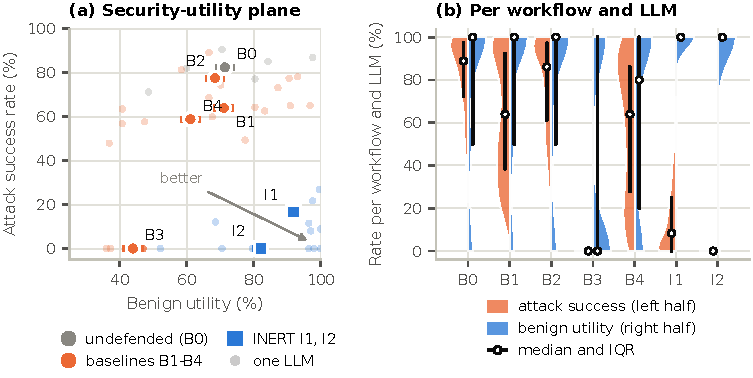
\includegraphics[width=\textwidth]{figures/fig_tradeoff.pdf}
\caption{Security and utility on the topology zoo. (a) Large markers are conditions with Wilson 95\% intervals on both axes, small markers single LLMs. (b) Split violins over all workflow--LLM combinations: attack success on the left, benign utility on the right, with median (white dot) and interquartile range (bar).}\label{fig:tradeoff}
\end{figure}

\subsection{RQ1: Propagation without a controller}

%<<rq1_text>>
Without a controller, an injection rarely stays with the agent that reads it. Figure~\ref{fig:propagation}a--c reports B0 by topology and size, with bootstrap 95\% bands. The number of infected agents grows with the number of agents in 5 of 5 topologies (chain from 1.7 to 3.3, debate from 2.0 to 4.3, hierarchical from 1.9 to 3.3, pcr from 0.9 to 1.1, star from 1.9 to 3.2). The blast radius, the share of all agent outputs that carry attacker content, falls with size in 5 of 5 topologies, because added agents dilute the transcript rather than escape it. The longest infected chains occur in debate8 (mean depth 4.14). Attack success is highest for star5 (98.1\%) and lowest for pcr3 (62.4\%). The planner--coder--reviewer workflow propagates least because only the coder writes the artifact that reaches the executor.

For the second clause of H1 we compare message tampering (A3) across topologies. It succeeds under B0 in 80.1\% of the tests on chains, against 90.7\% on star topologies, so chains do not amplify tampering. Figure~\ref{fig:propagation}d separates exposure from effect. Under I1 and I2 about as many agents carry attacker content as under the message-level defences, yet the attacks rarely or never reach an effect: the injected text is still read and repeated, but it stays in data fields.

\textbf{Answer to RQ1.} Injections propagate to several agents in every topology, and the absolute number of infected agents grows with team size. Hypothesis H1 holds for the count of infected agents but not for the share of outputs, which decreases with size, and its second clause, that chains amplify tampering, is not supported.
%<</rq1_text>>

\begin{figure}[tbp]
\centering
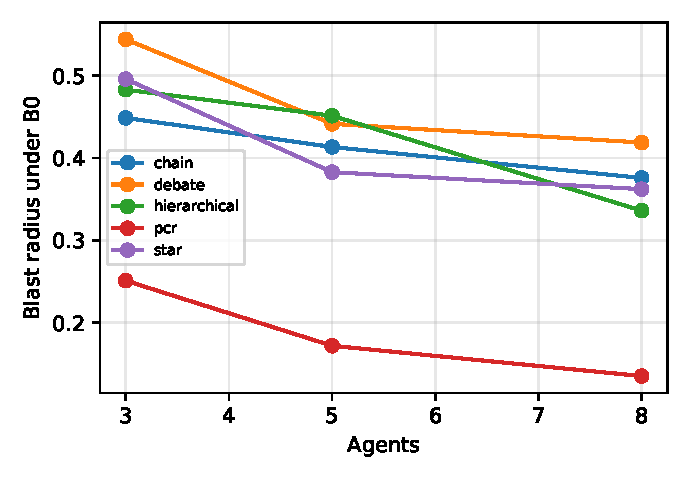
\includegraphics[width=\textwidth]{figures/fig_propagation.pdf}
\caption{RQ1. (a)--(c) Attack success, infected agents and infection depth under B0 by team size and topology, with bootstrap 95\% bands. (d) Exposure versus effect: mean infected agents per attacked run (bootstrap 95\% intervals), annotated with each condition's attack success rate.}\label{fig:propagation}
\end{figure}

\subsection{RQ2: Which mechanism blocks which attack}

%<<rq2_text>>
Figure~\ref{fig:ablation} reports the ablation suite (11{,}900 runs on 17 workflows with the four full-grid models), in which every INERT condition faces the same generated tests. I2 blocks every attacker model (the highest attack success over A1 to A5 is 0.0\%). Each ablation reopens precisely the channel that the taxonomy of Section~\ref{sec:taxonomy} assigns to it. Without tokens, compromised agents (100.0\%), message tampering (91.9\%) and colluding agents (100.0\%) succeed, because forged and altered proposals are accepted. These successes are audited authorship violations (P2): in none of them did the forged value also reach its goal in the sandbox, because selection and validators still bound what the forged value can steer. A rogue agent succeeds in all 16 of its tests (5.3\% of A5), because a registered agent can answer requests without a capability. Without key matching, A5 reaches 73.4\%: replayed proposals succeed in 70.5\% of the replay tests, and every one of the 68 tool-metadata tests succeeds, because our implementation ties the comparison of the run-time tool description with the pinned hash to the same switch (the pinned hash is part of the contract and therefore of the key). Without validators, colluding agents reach 100.0\% and a compromised executor agent 17.3\%; these successes reach their goal in the sandbox. Without any taint (I1), indirect injection succeeds in 20.4\% of the tests, which is the semantic propagation that structural mechanisms cannot see. A compromised agent also succeeds in 22.7\% of the tests under I1, but all 126 of these successes are SLOT tests in which the compromised agent writes the payload into its own slot, from where it travels semantically to the executor. Its attempts to answer another agent's request are all rejected. Colluding agents succeed in 50.0\% of the tests under I1 for the same reason: the middle agent's output, which carries the attacker's target, enters the executor's context once selection is off and then satisfies the grounding validator. Removing only one of the two taint checks keeps the attack success rate at zero, because selection and acceptance back each other up. They are not interchangeable, however. Without selection the executor agent sees tainted context, its proposals are rejected at acceptance, and the task fails: on the ablation suite, utility under attack is 0.0\% without selection against 56.4\% for I2 (Table~\ref{tab:main} reports 61.4\% for I2 on the full grid). Acceptance alone is the safety net if selection is misconfigured.

Figure~\ref{fig:ablation}b shows the first rejection in each I2 run. Under I2, 89\% of the A1 tests cause no rejection at all: selection withheld the tainted read, so the executor never proposed an injected value, and the attack failed without any check having to fire. In every A2 and A4 test the compromised agents first try to answer requests of other slots, which fails \textsc{Cap} (\textsc{TokenInvalid}), so this is the first rejection. Their proposals for their own slots carry valid tokens; they are rejected later by owned validators (272 \textsc{ValidatorReject} decisions in these runs) or accepted as data that selection keeps from the executor, which is why \textsc{ValidatorReject} does not appear as a first rejection. For A5, replays fail \textsc{Fresh} (63\%), altered tool metadata fails at tool execution (22\%, \textsc{ToolMetadataMismatch}) and proposals of a rogue agent fail \textsc{Cap} (14\%).

\textbf{Answer to RQ2.} Tokens stop authorship attacks, key matching stops replay (and, in our implementation, the use of altered tool metadata), validators bound the authority of compromised agents, and the taint policy is the only mechanism that stops semantic propagation into executor fields. H2 is supported, with one qualification: under I1 a compromised agent still wins through the semantic channel of its own output, which only the taint policy closes.
%<</rq2_text>>

\begin{figure}[tbp]
\centering
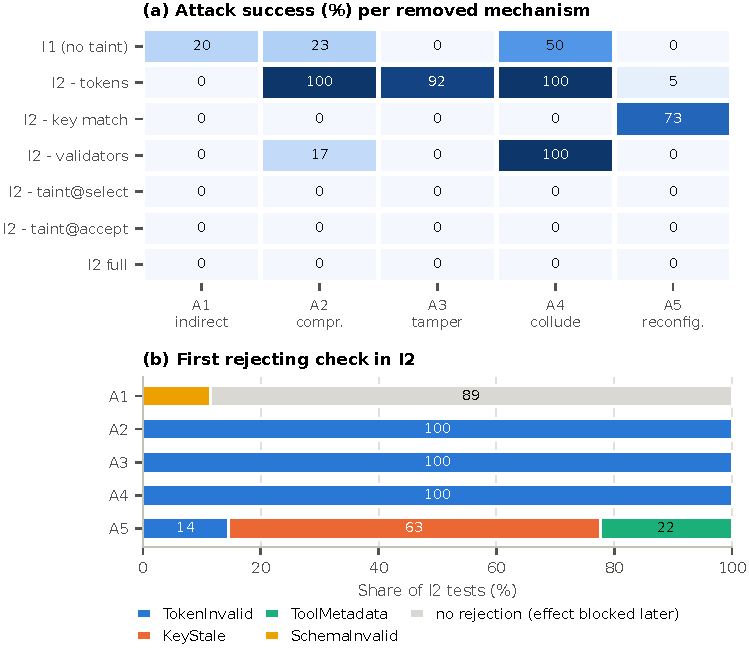
\includegraphics[width=\textwidth]{figures/fig_ablation.pdf}
\caption{RQ2. (a) Attack success rate per removed mechanism and attacker model. Each removal reopens the channel that Figure~\ref{fig:channel-tree} assigns to the mechanism. (b) First rejection in each I2 run per attacker model; later rejections in the same run, such as \textsc{ValidatorReject} for a compromised agent's own slot, are not shown. ``No rejection'': no proposal had to be rejected because selection withheld the tainted content or the effect was blocked at tool execution.}\label{fig:ablation}
\end{figure}

\subsection{RQ3: Model-based versus benchmark-style attack suites}

%<<rq3_text>>
Table~\ref{tab:rq3} compares the suites. The benchmark-style suites inject one payload into the primary untrusted resource, as AgentDojo and InjecAgent do. The generated suites cover the six criteria of Section~\ref{sec:generation} and were sampled to at most 15 tests per workflow and task (ten per workflow for the 70B-class models). Both suites are pooled in the $n_{att}$ of Table~\ref{tab:main}. Figure~\ref{fig:discovery}a--b plots how many distinct obligations each suite violates as the target spends LLM calls, averaged over 200 random orderings of the tests, and Figure~\ref{fig:discovery}c gives the attack success per criterion. Against B0 the generated suites yielded 88.6 successful attacks per 1{,}000 LLM calls against 77.8 for the benchmark-style suites, and violated 761 distinct obligations against 153. Against B4 the generated suites yielded 64.9 successful attacks per 1{,}000 LLM calls against 61.4 for the benchmark-style suites, and violated 712 distinct obligations against 147. Against B0 the most effective criterion is COLL (100.0\%), and the criteria that benchmarks do not cover, compromised and colluding agents and tampering in transit, are among the most effective, while benchmark-style injection ranks in the middle. Neither suite found a successful attack against I2, so the generated tests also act as a regression suite for the defence.

\textbf{Answer to RQ3.} At equal cost, model-coverage suites find more successful attacks and reach several times more distinct model elements than benchmark-style suites. H3 is supported.
%<</rq3_text>>

\begin{table}[tbp]
\caption{RQ3: generated and benchmark-style suites. Calls: LLM calls spent by the target. Succ./1k: successful attacks per 1{,}000 calls. Distinct: obligations with at least one successful attack.}\label{tab:rq3}
\scriptsize\setlength{\tabcolsep}{3pt}
%<<tab_rq3>>
\begin{tabular}{@{}llrrrrr@{}}
\toprule
Target & Suite & Tests & Succ. & Calls & Succ./1k & Distinct \\
\midrule
B0 & bench & 1530 & 1198 & 15392 & 77.83 & 153 \\
B0 & generated & 7140 & 5947 & 67156 & 88.56 & 761 \\
B4 & bench & 1530 & 917 & 14927 & 61.43 & 147 \\
B4 & generated & 7140 & 4182 & 64484 & 64.85 & 712 \\
I2 & bench & 1530 & 0 & 12510 & 0.00 & 0 \\
I2 & generated & 7140 & 0 & 47290 & 0.00 & 0 \\
\botrule
\end{tabular}
%<</tab_rq3>>
\end{table}

\begin{figure}[tbp]
\centering
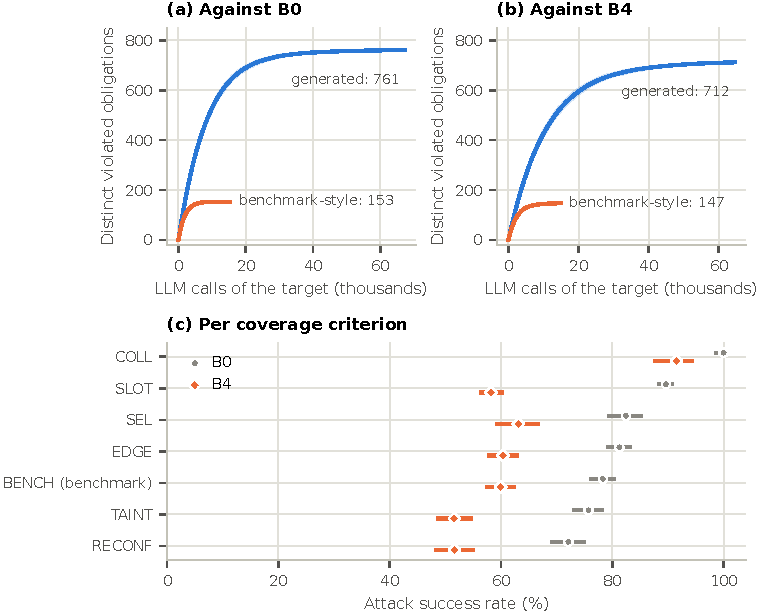
\includegraphics[width=\textwidth]{figures/fig_discovery.pdf}
\caption{RQ3. (a), (b) Distinct violated obligations as a function of the LLM calls spent by the target, averaged over 200 random orderings of each suite with 95\% bands. (c) Attack success per coverage criterion against B0 and B4 with Wilson 95\% intervals (no test succeeded against I2).}\label{fig:discovery}
\end{figure}

\subsection{RQ4: Cost}

%<<rq4_text>>
Table~\ref{tab:main} reports benign utility, false rejections and LLM calls, and Figure~\ref{fig:cost} the distributions of tokens and latency. I2 completes 82.2\% of benign tasks, which is more than B0 (71.4\%). The paired comparison gives an odds ratio of 2.43 for I2 succeeding where B0 fails versus the opposite (Holm-adjusted $p$ $<0.001$). This comparison, however, changes two factors at once: the coordination substrate (typed slots with one question each and a fixed schedule instead of a free-form group chat) and the security mechanisms. I1 uses the same substrate with tokens, keys and validators but without taint, so it separates the two. Typed slots raise benign utility from 71.4\% (B0) to 91.9\% (I1), and the taint policy then costs 9.7 points (I1 to I2). The cost falls on the code family (88.1\% under I1, 54.2\% under I2), where the coder sees only the declassified function name instead of the issue text. On reply, the declassified sender address keeps I2 at 81.6\% (80.6\% under I1; the declassifier fails when the planner picks the wrong e-mail), and on email and web I2 completes 100.0\% and 100.0\% of the tasks. B3 completes 0.0\% of the reply and 0.0\% of the code tasks, because its planner never sees the e-mail or issue it must act on. I2 rejects 1.1\% of honest proposals. B1 flags 2.0\% of benign messages, B3's policy blocks 25.2\% of attempted actions and B4's generated graph 54.0\%. On average I2 uses 8.2 LLM calls and 2{,}946 tokens per task against 10.0 and 5{,}424 for B0 (means; Figure~\ref{fig:cost} shows medians; Cliff's $\delta$ for tokens $-0.45$, for latency $-0.29$), because agents see only selected slot values instead of the whole transcript. I1 uses 3{,}072 tokens on average, so the savings come from slot-scoped context, not from taint.

Under attack, I2 keeps 61.4\% utility against 24.9\% for B0. The losses come from attacks against which INERT deliberately fails closed. A tampered proposal or a tool whose metadata changed is refused rather than used, which turns an integrity attack into an availability loss.

\textbf{Answer to RQ4.} Relative to the undefended system INERT's net utility is higher on our tasks, because typed slots help more than the taint policy costs; the cost of the security mechanisms proper is the 9.7-point gap between I1 and I2, much lower than B3's loss, and INERT's false-rejection rate is the lowest of all defences. H4 predicted a loss relative to B0 comparable to B3's, so the outcome is more favourable than hypothesized, and its second part (false rejections below B1's flag rate) holds.
%<</rq4_text>>

\begin{figure}[tbp]
\centering
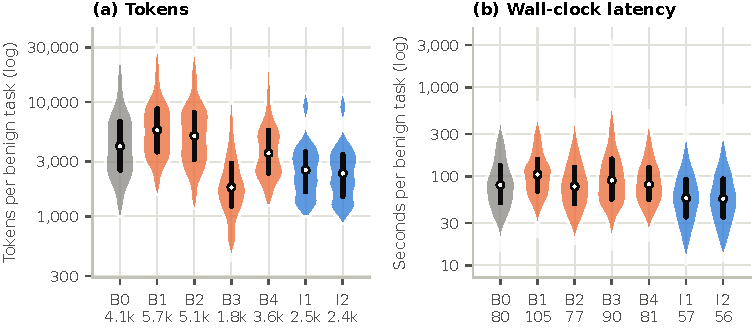
\includegraphics[width=\textwidth]{figures/fig_cost.pdf}
\caption{RQ4. Tokens and seconds per benign task (logarithmic scale) with median (white dot, value under each label) and interquartile range (bar).}\label{fig:cost}
\end{figure}

\subsection{Results per model and task family}\label{sec:per-model}

%<<llm_text>>
Table~\ref{tab:llm} breaks the main conditions down by model and Table~\ref{tab:family} benign utility by task family. I2's attack success rate is 0.0\% for every model, while B0's ranges from 71.2\% (\texttt{llama3.1:8b}) to 90.5\% (\texttt{qwen2.5:7b}), so the guarantee does not depend on how susceptible a model is. Utility does depend on the model: I2 completes between 52.2\% (\texttt{llama3.1:8b}) and 100.0\% (\texttt{qwen2.5:72b}) of benign tasks. The cost of the taint policy (I1 minus I2) is largest for \texttt{llama3.3:70b} (26.5 points) and smallest for \texttt{gemma2:9b} ($-0.4$ points). The difference lies in the code family, where the coder sees only the declassified function name instead of the issue: under I2, \texttt{llama3.1:8b} and \texttt{llama3.3:70b} complete no code task; \texttt{mistral-small:24b} 32.0\%, \texttt{qwen2.5:7b} 88.0\%; \texttt{gemma2:9b} and \texttt{qwen2.5:72b} complete all of them. On email, web and reply, I1 and I2 differ by at most 5.0 points for any model. The 70B-class models ran the reduced grid with two benign tasks per workflow, so their utility rests on fewer runs. B3 stays between 36.1\% and 47.1\% for every model, because its losses are structural: it completes no reply or code task. By task family, every condition does best on email and web, and the code family, whose executor needs the content of an untrusted issue, separates the conditions most.
%<</llm_text>>

\begin{table}[tbp]
\caption{Attack success rate and benign utility $U$ (\%) on the topology zoo per model. The 70B-class models ran the reduced grid (Section~\ref{sec:design}).}\label{tab:llm}
\scriptsize\setlength{\tabcolsep}{3pt}
%<<tab_llm>>
\begin{tabular}{@{}lrrrrrrrrrr@{}}
\toprule
 & \multicolumn{2}{c}{B0} & \multicolumn{2}{c}{B3} & \multicolumn{2}{c}{B4} & \multicolumn{2}{c}{I1} & \multicolumn{2}{c}{I2} \\
Model & ASR & $U$ & ASR & $U$ & ASR & $U$ & ASR & $U$ & ASR & $U$ \\
\midrule
\texttt{gemma2:9b} & 82.0 & 60.0 & 0.0 & 36.1 & 56.8 & 40.8 & 21.7 & 97.6 & 0.0 & 98.0 \\
\texttt{llama3.1:8b} & 71.2 & 48.6 & 0.0 & 47.1 & 47.9 & 36.9 & 12.0 & 68.6 & 0.0 & 52.2 \\
\texttt{llama3.3:70b} & 85.1 & 84.3 & 0.0 & 37.3 & 59.9 & 67.6 & 8.0 & 97.1 & 0.0 & 70.6 \\
\texttt{mistral-small:24b} & 86.9 & 97.6 & 0.0 & 47.1 & 65.0 & 91.0 & 11.5 & 96.5 & 0.0 & 79.6 \\
\texttt{qwen2.5:72b} & 77.1 & 80.4 & 0.0 & 47.1 & 49.3 & 77.5 & 8.9 & 100.0 & 0.0 & 100.0 \\
\texttt{qwen2.5:7b} & 90.5 & 70.6 & 0.0 & 47.1 & 68.6 & 66.7 & 26.9 & 99.6 & 0.0 & 96.5 \\
\botrule
\end{tabular}
%<</tab_llm>>
\end{table}

\begin{table}[tbp]
\caption{Benign utility (\%) on the topology zoo per task family, over all models. Reply and code workflows have a declassifier (Section~\ref{sec:design}).}\label{tab:family}
\footnotesize
%<<tab_family>>
\begin{tabular}{@{}lrrrrr@{}}
\toprule
Def. & email & reply & web & code & all \\
\midrule
B0 & 94.1 & 76.4 & 87.2 & 36.7 & 71.4 \\
B1 & 93.8 & 75.7 & 87.2 & 36.4 & 71.1 \\
B2 & 94.8 & 74.0 & 82.3 & 31.9 & 68.5 \\
B3 & 92.0 & 0.0 & 94.8 & 0.0 & 44.0 \\
B4 & 79.5 & 63.9 & 78.5 & 30.3 & 61.1 \\
I1 & 100.0 & 80.6 & 100.0 & 88.1 & 91.9 \\
I2 & 100.0 & 81.6 & 100.0 & 54.2 & 82.2 \\
\botrule
\end{tabular}
%<</tab_family>>
\end{table}

\subsection{RQ5: Adaptive attacker}

%<<rq5_text>>
Figure~\ref{fig:adaptive}a shows cumulative success as a function of the attempt budget. The adaptive attacker had ten attempts per case, the model description, the policy text and, after each attempt, the tools that were called and, for INERT, the controller's rejection reasons. Each condition faces 36 cases (nine workflows of size five, two tasks, two models); in the five code workflows the executor reads a regex declassifier of the issue, so the attacker could also try to pass a payload through a declassified value. Against B1 it succeeded in 88.9\% of 36 cases after 2.4 attempts on average. Against B3 it succeeded in 0.0\% of 36 cases, exhausting its budget. Against B4 it succeeded in 75.0\% of 36 cases after 3.6 attempts on average. Against I2 it succeeded in 0.0\% of 36 cases, exhausting its budget. Feedback helped the attacker against the message-level defences, which it learned to evade within a few attempts. Against I2 the rejection reasons only told the attacker that untrusted content never reaches the executor, which no payload can change.

\textbf{Answer to RQ5.} The structural and taint guarantees held under adaptive attack, including on the workflows with declassifiers. H5 is supported for the zoo: P1 to P6 held, and no residual success occurred, so its second clause could only be observed on TAMAS, where the residual successes (next subsection) come from authority that the model grants to agents. Ten attempts against bounded regular expressions do not establish the robustness of declassifiers against stronger attackers.
%<</rq5_text>>

\begin{figure}[tbp]
\centering
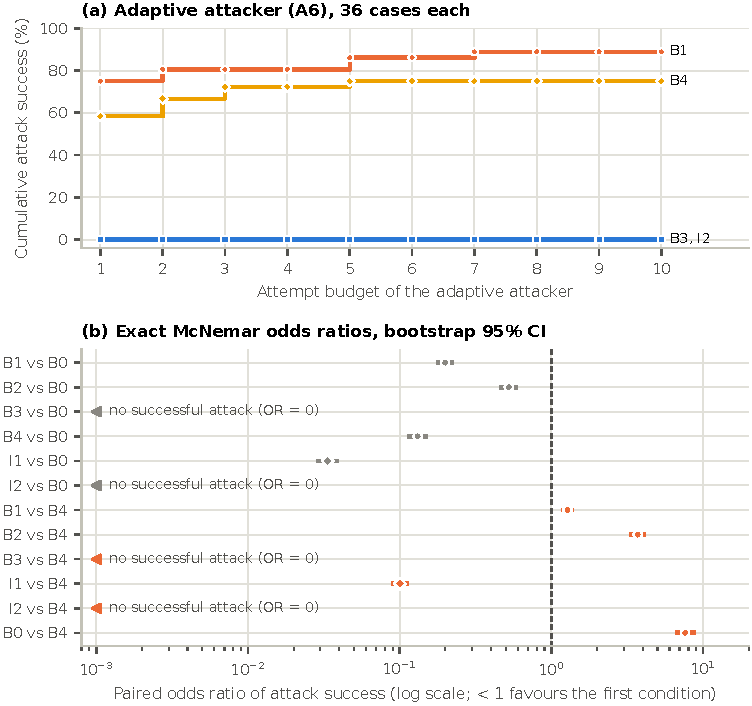
\includegraphics[width=\textwidth]{figures/fig_adaptive.pdf}
\caption{(a) RQ5: cumulative success of the adaptive attacker by attempt budget (B3 and I2 coincide at zero). (b) Exact McNemar tests on paired attack outcomes against B0 and B4: odds ratios with bootstrap 95\% intervals. Conditions without any successful attack have an odds ratio of zero and are marked at the left edge.}\label{fig:adaptive}
\end{figure}

\subsection{TAMAS}

%<<tamas_text>>
Table~\ref{tab:tamas} reports TAMAS, with 300 runs per cell (50 instances, six models). Indirect injection (IPI) succeeds in 51.7\% of instances under B0, 15.0\% under B4, 2.3\% under B3 and 8.0\% under I2. The TAMAS oracles cannot distinguish an attack-induced call from a call the task makes anyway: 23 of the 24 IPI successes under I2 are runs in which the benign run of the same instance and model calls the same target tool, which happens in 25 of 300 benign runs, so I2's IPI rate is at the oracle's floor rather than a flow of injected content. For direct injection, the outcome depends on what the system knows about provenance. When the whole query counts as the user's request (DPI-whole, as in TAMAS), I2 reaches 44.3\%, slightly below the range of the other conditions (45.7\% to 55.3\%), so INERT gives little protection here, because INERT trusts the user's channel by design. With the injected suffix labelled untrusted (DPI-split), I2 reaches 7.0\% against 55.0\% for B0 (17 of the 21 I2 successes coincide with the benign run), and impersonation, also delivered in the query, 28.7\%. DPI-split is an idealized setting: it assumes that the boundary between the user's text and the injected text is known, for instance because a user interface or protocol keeps attachments apart. INERT does not segment a prompt itself.

TAMAS agents carry harmful tools in their own tool sets, and Byzantine and colluding personas tell them to use these tools, which I2 does not prevent: Colluding reaches 10.3\% and Byzantine 29.0\%, against 9.7\% and 21.0\% for B0, so INERT is no better than the undefended system here. B3 and B4 do better because both derive a per-task allowlist from the request. A post-hoc variant (I2S) adds a task-scope slot that reads only the request and lists the tools the task needs, enforced by an owned validator. It brings Colluding to 0.0\% and Byzantine to 1.3\%, at a benign utility of 54.7\% against 73.0\% for I2, because the scope sometimes omits a needed tool. We report I2S separately because it was designed after seeing the results.
%<</tamas_text>>

\begin{table}[tbp]
\caption{TAMAS: attacker goal met (\%) per attack type and benign utility $U_{ben}$ (\%), 300 runs per cell (50 instances, six models). DPI-w/DPI-s: whole query labelled as user input or injected suffix labelled untrusted. Coll., Imp., Byz., Contr.: colluding, impersonation, Byzantine, contradicting agents. I2S: post-hoc task-scope variant.}\label{tab:tamas}
\scriptsize\setlength{\tabcolsep}{3pt}
%<<tab_tamas>>
\begin{tabular}{@{}lrrrrrrrr@{}}
\toprule
Def. & DPI-w & DPI-s & IPI & Coll. & Imp. & Byz. & Contr. & $U_{ben}$ \\
\midrule
B0 & 55.0 & 55.0 & 51.7 & 9.7 & 32.3 & 21.0 & 10.0 & 76.7 \\
B1 & 55.3 & 53.7 & 10.7 & 8.0 & 30.3 & 18.7 & 11.0 & 76.3 \\
B2 & 54.3 & 55.0 & 48.7 & 6.7 & 28.3 & 19.0 & 10.0 & 75.3 \\
B3 & 54.7 & 55.0 & 2.3 & 0.0 & 31.3 & 0.0 & 0.3 & 76.3 \\
B4 & 48.0 & 47.7 & 15.0 & 0.0 & 21.3 & 0.3 & 0.3 & 65.7 \\
I1 & 45.7 & 37.0 & 29.7 & 11.7 & 27.0 & 29.3 & 2.7 & 73.0 \\
I2 & 44.3 & 7.0 & 8.0 & 10.3 & 28.7 & 29.0 & 2.7 & 73.0 \\
I2S & 34.3 & 3.0 & 3.0 & 0.0 & 19.3 & 1.3 & 0.7 & 54.7 \\
\botrule
\end{tabular}
%<</tab_tamas>>
\end{table}

%=====================================================================================
\section{Discussion}\label{sec:discussion}

%<<discussion_text>>
\paragraph{Structural and semantic guarantees fail differently.} Tokens, key matching and metadata pinning defeat attacks on authorship, freshness and configuration whatever the payload says, so feedback does not help an adaptive attacker. The taint policy decides what an agent may see before the agent makes its decision, which is why only this policy stops an injected recipient, path or command from travelling into an executor field. Message-level defences, in contrast, judge single messages, whereas the harm arises from a flow across agents.

\paragraph{Where INERT does not help.} Residual risk sits in authority the model grants: a compromised owner of an executor field can misuse it within its validators, and content in the user's own request is trusted. Model-level least privilege such as the task scope of I2S narrows this risk but moves it to the component that decides the scope.

A rule-based categorization of the successful attacks against I2, derived from the run records, shows where the residual risk lies. None occurred on the topology zoo, so all are TAMAS runs. Because DPI-whole and DPI-split are two labelings of the same direct-injection runs, we count each TAMAS configuration separately. With the whole query trusted, as in TAMAS, there are 369 successes: 219 (59\%) arrived in the user's own request (direct injection or impersonation), 126 (34\%) were harmful tools in a compromised agent's own tool set, 24 (7\%) called a target tool that agents also call on benign runs (23 of them on the benign run of the same instance and model). With the injected suffix labelled untrusted, there are 257: 86 (33\%) arrived in the user's own request (impersonation), 126 (49\%) were harmful tools in a compromised agent's own tool set, 45 (18\%) called a target tool that agents also call on benign runs (40 of them on the benign run of the same instance and model).

\paragraph{Availability.} Failing closed turns tampering into refusals. This opens a denial-of-service surface, which an authenticated transport between agents and controller would remove.
%<</discussion_text>>

\paragraph{The taxonomy as a design and test instrument.} The channel tree predicted how each class of attack would fare. Structural forms closed by construction (RQ2, RQ5), semantic forms closed only through the taint checks, and residual forms remained where the model grants authority (TAMAS). The coverage criteria that benchmarks lack were also among the most effective (Figure~\ref{fig:discovery}c).

\paragraph{Implications.} Fields that steer tools should be bounded and fed from trusted inputs or declassifiers, and free text should flow only into data fields. Benchmarks should publish their workflows as models so that channel obligations can be derived from them, and evaluations should report the attack stages separately, because exposure and effect can differ widely (Figure~\ref{fig:propagation}d).

%=====================================================================================
\section{Threats to Validity}\label{sec:threats}

\paragraph{Construct validity.} Success is judged by sandbox effects plus audited violations. For the baselines, ASR includes a control-flow clause that also fires on many benign runs (Section~\ref{sec:results}), so we report the effect-only Goal rate beside it. For TAMAS, deterministic oracles and a harmful-tool heuristic replace the GPT-4o judge and cannot tell an attack-induced call from one the task makes anyway, and each instance runs as a fixed round-robin schedule of slots with our IPI payloads instead of TAMAS's conversational routing, so absolute TAMAS rates are not comparable with the original benchmark. Marker-based infection detection misses paraphrases and underestimates propagation.

For the taxonomy, the corpus depends on two queries, two databases and two citation indexes. Scopus citations were found by matching seed titles in reference lists, which can miss references with a different title and match unrelated ones, and for \NScOnly{} Scopus records without an OpenAlex entry screening relied on the title alone. Only \NScKnown{} of the \NScRule{} relevant Scopus records had been found before, so other indexes would add further studies. The link threshold of \NLinkK{} trades recall for focus and favours older, well-cited work (counts for every threshold are published). One author screened and classified the corpus (including the \NSnow{} snowballing and \NScopus{} Scopus studies) with the assistance of an LLM, so the screening and the classification have not been validated by an independent rater, and we report no inter-rater agreement. To make up for this in part, the criteria, the codebook, the cached raw data and every decision are published so that each step can be repeated.

\paragraph{Internal validity.} The baselines are reimplementations (B3 uses JSON plans instead of CaMeL's interpreter, which lowers its utility, and B4 omits ControlValve's per-edge rules and must infer the workflow graph from the request, which raises its false rejections) that share IR, models, tools and seeds with INERT. Only INERT has the designer's graph and owned validators; the I2-validator ablation isolates the validators, and I1 separates the typed-slot substrate from the taint policy (RQ4). Because the author also wrote the zoo models, they could favour INERT. We wrote them in the most direct style, in which every executor reads the final analysis, so the linter reports an untrusted path (L3) in every model and protection comes from the runtime rather than from the design of the model.

\paragraph{External validity.} We study moderate-size open-weight models and simulated tools across five domains and topologies, so results may differ for frontier models, real tools, other frameworks, long-running systems and persistent memory (C6).

\paragraph{Conclusion validity.} LLM outputs vary even at temperature 0. To account for this variation, we use paired tests, mixed models, bootstrap intervals and Holm correction, archive every record, and repeat a subset with five seeds at temperature 0.7.
%<<seeds_text>>
Across seeds, the standard deviation of the attack success rate is 0.6\% for B0, 2.9\% for B4, 0.0\% for I2, and the ordering of the conditions is the same for every seed.
%<</seeds_text>>

%=====================================================================================
\section{Related Work}\label{sec:related}

We compare INERT and its taxonomy with existing work along the branches of the corpus tree and the requirements of Table~\ref{tab:gaps}. Besides the corpus, this section draws on targeted searches for closely related work that we ran before the snowballing and that found 22 works. \NSuppSnow{} of them were later found independently by the snowballing and belong to the corpus. The other \NSupp{} did not inform the taxonomy and are listed separately in the replication package.

\subsection{Taxonomies of attacks, risks and failures}\label{sec:rw-tax}

Prompt-injection taxonomies classify attack techniques, from an exploratory checklist \citep{rossi2024categorization} to an ontology derived from 600,000 competition prompts \citep{schulhoff2023hackaprompt} and a formal composition of separator and injected task \citep{liu2024formalizing}. Agent-security surveys organize threats by knowledge gap, attack vector, protocol or attack path \citep{deng2025agentsthreat,Ferrag2025FromPIB,Wang2026TheLOT,Yang2026SoKWSJ}, multi-agent work by tiered or layered risks \citep{Mitra2026WhereREC,Wang2026TrinityGuardAUF} or failure modes such as collusion \citep{hammond2025multiagent}, MAST classifies functional failures from annotated traces \citep{cemri2025mast}, and practitioner frameworks catalogue threats with mitigations \citep{owasp2025agentic,mitre2025atlas}. As a methodological reference from software engineering we also include fault taxonomies such as that of \citet{humbatova2020taxonomy}, which are built empirically and validated with practitioners as testing checklists.

\begin{table}[tbp]
\caption{Taxonomies related to ours. Mech.: categories mapped to enforcement mechanisms. Tests: categories mapped to test obligations or test data. \cfull: for every category. \chalf: partly or indirectly. \cnone: no.}\label{tab:taxcmp}
\scriptsize\setlength{\tabcolsep}{3pt}
\begin{tabular*}{\textwidth}{@{\extracolsep\fill}L{2.75cm}L{2.55cm}L{1.75cm}L{3.0cm}cc@{}}
\toprule
Taxonomy & Classifies & Scope & Evidence base & Mech. & Tests \\
\midrule
Rossi et al. \citep{rossi2024categorization} & attack techniques & LLM apps & exploratory review & \cnone & \cnone \\\addlinespace[1.2pt]
HackAPrompt \citep{schulhoff2023hackaprompt} & prompt-hacking techniques & single LLM & 600K contest prompts & \cnone & \chalf \\\addlinespace[1.2pt]
Liu et al. \citep{liu2024formalizing} & attack compositions & LLM apps & formal framework, benchmark & \chalf & \chalf \\\addlinespace[1.2pt]
Agent-security surveys, SoK \citep{deng2025agentsthreat,Ferrag2025FromPIB,Wang2026TheLOT,Yang2026SoKWSJ} & threats, vectors, attack paths & agents, MAS & literature surveys & \chalf & \cnone \\\addlinespace[1.2pt]
Mitra et al., TrinityGuard \citep{Mitra2026WhereREC,Wang2026TrinityGuardAUF} & risk tiers, rule vs.\ judge boundary, layered risks & MAS & framework, evaluation & \chalf & \chalf \\\addlinespace[1.2pt]
Hammond et al. \citep{hammond2025multiagent} & failure modes, risk factors & advanced MAS & expert analysis & \cnone & \cnone \\\addlinespace[1.2pt]
MAST \citep{cemri2025mast} & functional failure modes & MAS & annotated traces, $\kappa = 0.88$ & \cnone & \chalf \\\addlinespace[1.2pt]
OWASP, MITRE ATLAS \citep{owasp2025agentic,mitre2025atlas} & threats, tactics, mitigations & agents, AI & practice, case studies & \chalf & \cnone \\\addlinespace[1.2pt]
Humbatova et al. \citep{humbatova2020taxonomy} & real faults & DL systems & 1,059 artefacts, interviews & \cnone & \chalf \\\addlinespace[1.2pt]
\midrule
This paper & handoffs by receiving interface & MAS & \NCorpus{} studies, audit & \cfull & \cfull \\\addlinespace[1.2pt]
\botrule
\end{tabular*}
\end{table}

Table~\ref{tab:taxcmp} compares these taxonomies with ours on four dimensions. In \emph{unit}, they classify techniques, threats, risks or failures, while ours classifies handoffs by receiving interface, where a check can be inserted. In \emph{actionability}, they attach mitigations in prose, while each of our leaves names a mechanism and the property it guarantees. In \emph{testability}, only benchmark-derived taxonomies come with test data, and none maps categories to coverage criteria as our tree does. In \emph{evidence}, our corpus is collected reproducibly and published with an audit trail, but unlike MAST and \citet{humbatova2020taxonomy} our classification has not been validated by independent raters or practitioners, which remains a threat to validity. The taxonomies are complementary: technique taxonomies describe payloads, MAST describes cooperative failures, and ours describes where to mediate and what to test.

Several taxonomies and surveys in our corpus organize the field by protocol or by layer, among them attack vectors in the Model Context Protocol ecosystem \citep{Song2025BeyondTPAE}, threats from prompt injection to protocol exploits in agent workflows \citep{Ferrag2025FromPIB}, a layered review of agent frameworks \citep{Xu2026SecurityAAJ} and threat taxonomies for agent skills \citep{Li2026TowardsSABM}. Their protocol-level categories fall mostly into our channels C3 and C7, where content arrives as a tool response or as discovery metadata. Surveys of prompt injection in LLM applications \citep{Cao2026ASSM,Geng2025PromptIABB,Rababah2024SoKPHBH,McHugh2025PromptI2F} catalogue techniques that our payload classes and mutators sample, and surveys and position papers on agent security \citep{Witt2025OpenCIBE,Siu2026AgentSNZ,Xiang2026ArchitectingSAAP,Ling2026TowardSLG} motivate system-level defences, the design space that our requirements R1 to R8 make explicit for workflows of several agents.

\subsection{Threats and propagation in multi-agent systems}

Injections replicate \citep{lee2024promptinfection}, hijack orchestration \citep{triedman2025mas}, travel through intercepted messages \citep{he2025aitm}, compose from fragments \citep{arif2026conjunctive}, bypass distributed safety mechanisms \citep{shahroz2025siege} and leak data through orchestrators \citep{naik2026omnileak}. Manipulated knowledge spreads and persists \citep{ju2024flooding}, faulty agents degrade collaboration by structure \citep{huang2025faulty}, and team shape changes exposure \citep{hagag2026architecture,Yu2025NetSafeETBB}. Work on topology models how injections and errors spread: as cross-layer contagion in agent swarms \citep{Le2026CrosslayerCOAI}, as error cascades in collaboration \citep{Xie2026FromSTBA}, and as a function of roles and topological structure \citep{Zhu2025MASTERMSR} or of the move from monolithic agents to swarms \citep{Malla2026FromMTI}. RQ1 adds a controlled measurement of propagation and of the gap between exposure and effect.

Most attack mechanisms in the corpus target a channel that INERT mediates. Optimized or learned payloads, such as execution triggers learned for prompt injection \citep{Pasquini2024NeuralELAL}, reinforcement learning for injection \citep{Wen2025RLIAU} and images that jailbreak multimodal agents \citep{Gu2024AgentSAAO}, are stronger than our fixed payload classes and our adaptive attacker. They act on the content of data fields, which INERT does not judge, so the effect they can reach is bounded by the same labels and validators. Multi-round tampering of inter-agent messages \citep{Yan2025AttackTMAQ} targets C4 and fails against request-bound MACs. Registration-time injection through deceptive self-descriptions in centralized systems \citep{Yu2026MisleadingTPO} and injection into tool selection \citep{Shi2025PromptIAR} target C7. In INERT, registration grants no slot, tool descriptions are pinned by hash, and where an agent selects a tool it chooses a member of an enumeration fixed by the model. Memory poisoning \citep{Chen2024AgentPoisonRLBS,Sunil2026MemoryPABF} and cross-user poisoning \citep{Patlan2025CrossUserPUAK} use cross-session shared state (C6, gap G5), which INERT does not mediate. Attacks that end in SQL injection \citep{Pedro2023FromPIBE}, leakage of intellectual property \citep{Wang2025IPLAX} or private data \citep{Kao2026YouTMAZ}, or physical actions of robots \citep{Nagaraja2026WhenPCBF} reach executor sinks, the fields that our sink roles single out. Studies of trust boundaries report that security measures trade off against collaboration \citep{peigne2025securitytax} and that stronger LLM auditors can make a system less secure \citep{Liu2026TheCPT}, two observations that our results echo: a learned check is a new target, and INERT's utility cost is concentrated where untrusted content is needed. Finally, studies of deployed and shared workflows, such as software development teams \citep{Wang2025ShadowsITAL}, enterprise cyber operations \citep{Mitra2026AgenticCyOpsSMAH} and blackboard architectures \citep{Nakamura2025TerrariumRTAR}, show that the designer-defined workflows that INERT assumes exist in practice.

\subsection{Defences}

\paragraph{Learned and prompt-level defences.} Guard models \citep{inan2023llamaguard,li2025piguard}, activation-based detection of task drift \citep{abdelnabi2025drift}, detection by masked re-execution \citep{zhu2025melon} and prompt-level or training defences \citep{hines2024spotlighting,chen2025struq,wallace2024hierarchy,chen2025secalign} lower attack success with learned judgments (G1), which our adaptive attacker evaded within a few attempts. The same holds for detectors specific to multi-agent systems, which judge activations \citep{Xu2026WhenAGQ}, intention-hiding agents \citep{Xie2025WhosTMAI}, simulated communication states \citep{Shi2026SAIGuardCSN} or reconstructed semantic flows \citep{Cai2026CrossLayerSFBK}, use sentinel agents \citep{Gosmar2025SentinelAFAJ}, rectify sentences \citep{Luo2026DefendingLMV}, remediate along propagation paths \citep{Yan2026PropGuardSLAE}, or shield and guard the whole system \citep{Wang2025MASShieldADAF,Kachuee2026MASGuardUGW}. MESA prioritizes vulnerable communication channels for securing a system \citep{Li2026MESAPVAS}, which is close in spirit to our channel-derived obligations but serves defence placement rather than test generation. Task-specific fine-tuning \citep{Piet2023JatmoPIAS} and guardrails that reduce over-defence \citep{Li2024InjecGuardBABC} improve the models themselves. All of these can run inside INERT's data fields, where they lower the chance that an agent writes a misleading value, while INERT bounds what such a value can steer.

\paragraph{Plan, flow and privilege control for agents.} CaMeL \citep{debenedetti2025camel}, the design patterns of \citet{beurerkellner2025patterns}, FIDES \citep{wu2024ifc}, DRIFT \citep{li2025drift}, IPIGuard \citep{an2025ipiguard} and RTBAS \citep{zhong2025rtbas} fix the plan before untrusted data is read or track information flow through tool calls. ACE separates abstract planning from concrete binding and checks plans against information-flow constraints \citep{li2026ace}. IsolateGPT isolates apps behind a trusted hub \citep{wu2025isolategpt}, Progent expresses tool privileges in a policy language \citep{shi2025progent}, Prompt Flow Integrity separates trusted and untrusted agents \citep{kim2025pfi}, and Conseca generates deterministic, context-specific policies \citep{tsai2025conseca}. INERT shares their deterministic enforcement but takes its policy from a designer-authored model of the whole workflow, mediates the channels between agents including authorship, freshness and coordination signals (G2, G3), and logs decisions for third-party replay (R7). Two further lines of work concern the execution boundary and the audit. Twin Agent compresses context for privilege-separated agents \citep{Hu2026TwinACI}, and studies of coding agents survey isolation and access control at the execution boundary \citep{Rashidi2026TheBOBQ}; INERT's fail-closed tool executor and sandbox belong to this boundary, but its decisions are taken before a tool runs. On the audit side, runtime verification has a long tradition for agent-oriented programming \citep{Engelmann2022RV4JaCaRBL}, and resilience of multi-agent control systems to attacks on communication has been studied in cyber-physical settings \citep{Taheri2020MitigationARBP}. INERT's replay audit is a runtime verifier whose monitored properties P1 to P6 are derived from the same model that the controller enforces.

\paragraph{Defences for multi-agent systems.} ControlValve enforces an LLM-generated control-flow graph \citep{jha2025controlvalve}, graph-based and collaborative monitors filter or prune malicious agents \citep{Wang2025GSafeguardATAW,Miao2025BlindGuardSLAV,zeng2024autodefense}, AgentSafe restricts information by hierarchy \citep{Mao2025AgentSafeSLY}, and identity frameworks bind agents to verifiable identities or access control \citep{Zou2025BlockA2ATSAC,Narajala2025SecuringGMAU,Ji2026TamingVPAP} or treat the propagation of authorization as identity governance \citep{Tallam2026AuthorizationPIBH}. These bind an \emph{agent} to an identity; INERT additionally binds each \emph{value} to the request it answers, which is what freshness and replay protection need. Each covers a subset of R1 to R7 (Table~\ref{tab:gaps}). We compare against reimplementations of ControlValve (B4) and of the detection family (B1); Section~\ref{sec:design} explains why the learned multi-agent monitors and AgentSafe were not reimplemented.

\subsection{Evaluation, testing and model-driven security}

Benchmarks for single agents \citep{debenedetti2024agentdojo,zhan2024injecagent,zhang2025asb}, web agents \citep{evtimov2025wasp}, harmful agent behaviour \citep{andriushchenko2025agentharm} and multi-agent systems \citep{kavathekar2025tamas,An2026ACIArenaTUH} provide valuable scenarios but fix their injection points, and structural coverage criteria for agentic workflows \citep{kahani2026structural} derive obligations from the workflow's structure rather than from injection channels. Our generator complements both (G4), and RQ3 shows that channel-derived injection points find more distinct weaknesses at equal cost. WASP \citep{evtimov2025wasp} also reports injections that start but do not complete, which corresponds to our distinction between exposure and effect. Multi-agent evaluation frameworks benchmark debate \citep{Liu2026MADBenchBTU}, graph-based anomaly monitors \citep{MateoTorrejon2026GAMMAFACAG}, psychological attacks on agents \citep{Zhang2024PsySafeACAN}, red-teaming for injection detection \citep{Ogunjinmi2026AgenticARN} and safety and security more broadly \citep{Hagag2026ORBITAFAD,Sharma2025TowardsUQBD}. Large public competitions measure how often agents follow indirect injections \citep{Dziemian2026HowVAAN,Zou2025SecurityCIAD}, and model-level benchmarks cover indirect injection \citep{Yi2023BenchmarkingADAR}, long contexts \citep{Liu2026LongPIBenchALAV}, game-derived attacks \citep{Toyer2023TensorTIAM} and cybersecurity risks \citep{Wan2024CYBERSECEVAL3ABJ}. These benchmarks supply scenarios and payloads. If they published their workflows as models, our generator could derive channel obligations for them, and our effect oracles and audit would separate exposure from effect without an LLM judge.

Model-driven security \citep{lodderstedt2002secureuml,jurjens2002umlsec,basin2006mds} and model-based security testing \citep{utting2012taxonomy,felderer2016mbst} derive enforcement and tests from models. INERT applies both to systems whose components, the LLM agents, are untrusted, using a slot-level lattice policy \citep{denning1976lattice,sabelfeld2003language}, and derives enforcement and test obligations from one and the same model.

%=====================================================================================
\section{Conclusion}\label{sec:conclusion}

%<<conclusion_text>>
INERT treats an LLM multi-agent system as a model-driven artifact. A taxonomy of seven injection channels determines what must be mediated, and one compiled model is enforced by a controller that acts as a reference monitor, tested by generated attacks and audited from a replayable log. The full configuration reduced attack success on the topology zoo to 0.0\% while completing 82.2\% of benign tasks, more than the undefended system and far more than the strongest design-level baseline, and model-derived suites exposed more weaknesses than benchmark-style attacks. The remaining risk lies in authority the model grants and in content that arrives as the user's own request. Future work will study how developers write INERT models, how task scopes can be given guarantees and how long-lived memory can be mediated.
%<</conclusion_text>>

\backmatter

\section*{Declaration of generative AI}
During the preparation of this work the author used \texttt{Claude Opus 5.5} in order to assist with organizing the repository code, drafting experiment and analysis scripts, screening the studies found by snowballing and in Scopus and assigning them to the leaves of the taxonomy codebook (Section~\ref{sec:tax-collection}), and checking the manuscript for grammatical errors. After using these tools, the author reviewed and edited the content as needed and takes full responsibility for the accuracy and integrity of all claims, references and the content of the published article.

\section*{Declarations}

\begin{itemize}
\item Funding: Not applicable.
\item Conflict of interest: The author declares no competing interests.
\item Ethics approval and consent to participate: Not applicable. No human participants were involved.
\item Consent for publication: Not applicable.
\item Data availability: All result records are in the repository (\texttt{results/final}), and the replication package (\texttt{docs/paper/EMSE/replication-package}) contains checksums, the scripts that regenerate every table, figure and number, and a mapping of the approach and the taxonomy to the code.
\item Materials availability: MAS models, attack suites, payload libraries and the corpus classification are part of the replication package. Payloads target only reserved example domains and carry a dual-use notice.
\item Code availability: \url{https://github.com/ai4se4ai/inert-mas}.
\item Author contribution: Not applicable (single author).
\end{itemize}

\bibliography{references}

\end{document}
